\documentclass{article}
\usepackage[final]{neurips_2025}  % NEURIPS style (neurips_2025.sty is in paper_draft/)
% neurips_2025.sty leaves \@trackname undefined without a track option; keep the notice empty
\makeatletter\providecommand{\@trackname}{}\makeatother
\usepackage[hidelinks]{hyperref}  % REQUIRED: clickable links
\usepackage{booktabs}  % REQUIRED: professional tables
\usepackage{graphicx}
\usepackage{amsmath,amssymb}
\usepackage[utf8]{inputenc}
\usepackage[T1]{fontenc}
\usepackage{enumitem}
\usepackage{multirow}
\usepackage{caption}
\usepackage{algorithm}
\usepackage[noend]{algpseudocode}

% Import command files
%%%%% MATH NOTATION MACROS %%%%%
% Standard math notation for academic papers
% Import with: %%%%% MATH NOTATION MACROS %%%%%
% Standard math notation for academic papers
% Import with: %%%%% MATH NOTATION MACROS %%%%%
% Standard math notation for academic papers
% Import with: \input{commands/math}

\usepackage{amsmath,amsfonts,bm}

%%%%%%%%%%%%%%%%%%%%%%%%%%%%%%%%%%%%%%%%%%%%%%%%%%%%%%%%%%%%%%%%%
% FIGURE AND SECTION REFERENCES
%%%%%%%%%%%%%%%%%%%%%%%%%%%%%%%%%%%%%%%%%%%%%%%%%%%%%%%%%%%%%%%%%

% Mark sections of captions for referring to divisions of figures
\newcommand{\figleft}{{\em (Left)}}
\newcommand{\figcenter}{{\em (Center)}}
\newcommand{\figright}{{\em (Right)}}
\newcommand{\figtop}{{\em (Top)}}
\newcommand{\figbottom}{{\em (Bottom)}}
\newcommand{\captiona}{{\em (a)}}
\newcommand{\captionb}{{\em (b)}}
\newcommand{\captionc}{{\em (c)}}
\newcommand{\captiond}{{\em (d)}}

% Figure references
\def\figref#1{figure~\ref{#1}}
\def\Figref#1{Figure~\ref{#1}}
\def\twofigref#1#2{figures \ref{#1} and \ref{#2}}
\def\quadfigref#1#2#3#4{figures \ref{#1}, \ref{#2}, \ref{#3} and \ref{#4}}

% Section references
\def\secref#1{section~\ref{#1}}
\def\Secref#1{Section~\ref{#1}}
\def\twosecrefs#1#2{sections \ref{#1} and \ref{#2}}
\def\secrefs#1#2#3{sections \ref{#1}, \ref{#2} and \ref{#3}}

% Equation references
\def\eqref#1{equation~\ref{#1}}
\def\Eqref#1{Equation~\ref{#1}}
\def\plaineqref#1{\ref{#1}}

% Algorithm references
\def\algref#1{algorithm~\ref{#1}}
\def\Algref#1{Algorithm~\ref{#1}}
\def\twoalgref#1#2{algorithms \ref{#1} and \ref{#2}}
\def\Twoalgref#1#2{Algorithms \ref{#1} and \ref{#2}}

% Table references
\def\tabref#1{table~\ref{#1}}
\def\Tabref#1{Table~\ref{#1}}

% Chapter references
\def\chapref#1{chapter~\ref{#1}}
\def\Chapref#1{Chapter~\ref{#1}}

%%%%%%%%%%%%%%%%%%%%%%%%%%%%%%%%%%%%%%%%%%%%%%%%%%%%%%%%%%%%%%%%%
% BASIC MATH DEFINITIONS
%%%%%%%%%%%%%%%%%%%%%%%%%%%%%%%%%%%%%%%%%%%%%%%%%%%%%%%%%%%%%%%%%

\def\ceil#1{\lceil #1 \rceil}
\def\floor#1{\lfloor #1 \rfloor}
\def\1{\bm{1}}
\def\eps{{\epsilon}}

% Common operators
\DeclareMathOperator*{\argmax}{arg\,max}
\DeclareMathOperator*{\argmin}{arg\,min}
\DeclareMathOperator{\sign}{sign}
\DeclareMathOperator{\Tr}{Tr}
\let\ab\allowbreak

%%%%%%%%%%%%%%%%%%%%%%%%%%%%%%%%%%%%%%%%%%%%%%%%%%%%%%%%%%%%%%%%%
% VECTORS (lowercase bold)
%%%%%%%%%%%%%%%%%%%%%%%%%%%%%%%%%%%%%%%%%%%%%%%%%%%%%%%%%%%%%%%%%

\def\vzero{{\bm{0}}}
\def\vone{{\bm{1}}}
\def\vmu{{\bm{\mu}}}
\def\vtheta{{\bm{\theta}}}
\def\va{{\bm{a}}}
\def\vb{{\bm{b}}}
\def\vc{{\bm{c}}}
\def\vd{{\bm{d}}}
\def\ve{{\bm{e}}}
\def\vf{{\bm{f}}}
\def\vg{{\bm{g}}}
\def\vh{{\bm{h}}}
\def\vi{{\bm{i}}}
\def\vj{{\bm{j}}}
\def\vk{{\bm{k}}}
\def\vl{{\bm{l}}}
\def\vm{{\bm{m}}}
\def\vn{{\bm{n}}}
\def\vo{{\bm{o}}}
\def\vp{{\bm{p}}}
\def\vq{{\bm{q}}}
\def\vr{{\bm{r}}}
\def\vs{{\bm{s}}}
\def\vt{{\bm{t}}}
\def\vu{{\bm{u}}}
\def\vv{{\bm{v}}}
\def\vw{{\bm{w}}}
\def\vx{{\bm{x}}}
\def\vy{{\bm{y}}}
\def\vz{{\bm{z}}}

%%%%%%%%%%%%%%%%%%%%%%%%%%%%%%%%%%%%%%%%%%%%%%%%%%%%%%%%%%%%%%%%%
% MATRICES (uppercase bold)
%%%%%%%%%%%%%%%%%%%%%%%%%%%%%%%%%%%%%%%%%%%%%%%%%%%%%%%%%%%%%%%%%

\def\mA{{\bm{A}}}
\def\mB{{\bm{B}}}
\def\mC{{\bm{C}}}
\def\mD{{\bm{D}}}
\def\mE{{\bm{E}}}
\def\mF{{\bm{F}}}
\def\mG{{\bm{G}}}
\def\mH{{\bm{H}}}
\def\mI{{\bm{I}}}
\def\mJ{{\bm{J}}}
\def\mK{{\bm{K}}}
\def\mL{{\bm{L}}}
\def\mM{{\bm{M}}}
\def\mN{{\bm{N}}}
\def\mO{{\bm{O}}}
\def\mP{{\bm{P}}}
\def\mQ{{\bm{Q}}}
\def\mR{{\bm{R}}}
\def\mS{{\bm{S}}}
\def\mT{{\bm{T}}}
\def\mU{{\bm{U}}}
\def\mV{{\bm{V}}}
\def\mW{{\bm{W}}}
\def\mX{{\bm{X}}}
\def\mY{{\bm{Y}}}
\def\mZ{{\bm{Z}}}
\def\mBeta{{\bm{\beta}}}
\def\mPhi{{\bm{\Phi}}}
\def\mLambda{{\bm{\Lambda}}}
\def\mSigma{{\bm{\Sigma}}}

%%%%%%%%%%%%%%%%%%%%%%%%%%%%%%%%%%%%%%%%%%%%%%%%%%%%%%%%%%%%%%%%%
% CALLIGRAPHIC (mathcal)
%%%%%%%%%%%%%%%%%%%%%%%%%%%%%%%%%%%%%%%%%%%%%%%%%%%%%%%%%%%%%%%%%

\def\gA{{\mathcal{A}}}
\def\gB{{\mathcal{B}}}
\def\gC{{\mathcal{C}}}
\def\gD{{\mathcal{D}}}
\def\gE{{\mathcal{E}}}
\def\gF{{\mathcal{F}}}
\def\gG{{\mathcal{G}}}
\def\gH{{\mathcal{H}}}
\def\gI{{\mathcal{I}}}
\def\gJ{{\mathcal{J}}}
\def\gK{{\mathcal{K}}}
\def\gL{{\mathcal{L}}}
\def\gM{{\mathcal{M}}}
\def\gN{{\mathcal{N}}}
\def\gO{{\mathcal{O}}}
\def\gP{{\mathcal{P}}}
\def\gQ{{\mathcal{Q}}}
\def\gR{{\mathcal{R}}}
\def\gS{{\mathcal{S}}}
\def\gT{{\mathcal{T}}}
\def\gU{{\mathcal{U}}}
\def\gV{{\mathcal{V}}}
\def\gW{{\mathcal{W}}}
\def\gX{{\mathcal{X}}}
\def\gY{{\mathcal{Y}}}
\def\gZ{{\mathcal{Z}}}

%%%%%%%%%%%%%%%%%%%%%%%%%%%%%%%%%%%%%%%%%%%%%%%%%%%%%%%%%%%%%%%%%
% SETS (blackboard bold)
%%%%%%%%%%%%%%%%%%%%%%%%%%%%%%%%%%%%%%%%%%%%%%%%%%%%%%%%%%%%%%%%%

\def\sA{{\mathbb{A}}}
\def\sB{{\mathbb{B}}}
\def\sC{{\mathbb{C}}}
\def\sD{{\mathbb{D}}}
\def\sF{{\mathbb{F}}}
\def\sG{{\mathbb{G}}}
\def\sH{{\mathbb{H}}}
\def\sI{{\mathbb{I}}}
\def\sJ{{\mathbb{J}}}
\def\sK{{\mathbb{K}}}
\def\sL{{\mathbb{L}}}
\def\sM{{\mathbb{M}}}
\def\sN{{\mathbb{N}}}
\def\sO{{\mathbb{O}}}
\def\sP{{\mathbb{P}}}
\def\sQ{{\mathbb{Q}}}
\def\sR{{\mathbb{R}}}
\def\sS{{\mathbb{S}}}
\def\sT{{\mathbb{T}}}
\def\sU{{\mathbb{U}}}
\def\sV{{\mathbb{V}}}
\def\sW{{\mathbb{W}}}
\def\sX{{\mathbb{X}}}
\def\sY{{\mathbb{Y}}}
\def\sZ{{\mathbb{Z}}}

%%%%%%%%%%%%%%%%%%%%%%%%%%%%%%%%%%%%%%%%%%%%%%%%%%%%%%%%%%%%%%%%%
% COMMON MATH SHORTCUTS
%%%%%%%%%%%%%%%%%%%%%%%%%%%%%%%%%%%%%%%%%%%%%%%%%%%%%%%%%%%%%%%%%

% Expectation and variance
\newcommand{\E}{\mathbb{E}}
\newcommand{\Var}{\mathrm{Var}}
\newcommand{\Cov}{\mathrm{Cov}}
\newcommand{\R}{\mathbb{R}}

% Datasets
\newcommand{\train}{\mathcal{D}}
\newcommand{\valid}{\mathcal{D_{\mathrm{valid}}}}
\newcommand{\test}{\mathcal{D_{\mathrm{test}}}}

% Distributions
\newcommand{\laplace}{\mathrm{Laplace}}
\newcommand{\Uniform}{\mathrm{Unif}}
\newcommand{\Normal}{\mathrm{Normal}}
\newcommand{\Categorical}{\mathrm{Categorical}}

% Common functions
\newcommand{\softmax}{\mathrm{softmax}}
\newcommand{\sigmoid}{\sigma}
\newcommand{\KL}{D_{\mathrm{KL}}}

% Norms
\newcommand{\normlzero}{L^0}
\newcommand{\normlone}{L^1}
\newcommand{\normltwo}{L^2}
\newcommand{\normlp}{L^p}
\newcommand{\normmax}{L^\infty}

%%%%%%%%%%%%%%%%%%%%%%%%%%%%%%%%%%%%%%%%%%%%%%%%%%%%%%%%%%%%%%%%%
% DEFINITIONS AND HIGHLIGHTING
%%%%%%%%%%%%%%%%%%%%%%%%%%%%%%%%%%%%%%%%%%%%%%%%%%%%%%%%%%%%%%%%%

% Highlight a newly defined term
\newcommand{\newterm}[1]{{\bf #1}}
\newcommand{\defn}[1]{\textbf{#1}}
\newcommand{\defeq}{\mathrel{\stackrel{\textnormal{\tiny def}}{=}}}


\usepackage{amsmath,amsfonts,bm}

%%%%%%%%%%%%%%%%%%%%%%%%%%%%%%%%%%%%%%%%%%%%%%%%%%%%%%%%%%%%%%%%%
% FIGURE AND SECTION REFERENCES
%%%%%%%%%%%%%%%%%%%%%%%%%%%%%%%%%%%%%%%%%%%%%%%%%%%%%%%%%%%%%%%%%

% Mark sections of captions for referring to divisions of figures
\newcommand{\figleft}{{\em (Left)}}
\newcommand{\figcenter}{{\em (Center)}}
\newcommand{\figright}{{\em (Right)}}
\newcommand{\figtop}{{\em (Top)}}
\newcommand{\figbottom}{{\em (Bottom)}}
\newcommand{\captiona}{{\em (a)}}
\newcommand{\captionb}{{\em (b)}}
\newcommand{\captionc}{{\em (c)}}
\newcommand{\captiond}{{\em (d)}}

% Figure references
\def\figref#1{figure~\ref{#1}}
\def\Figref#1{Figure~\ref{#1}}
\def\twofigref#1#2{figures \ref{#1} and \ref{#2}}
\def\quadfigref#1#2#3#4{figures \ref{#1}, \ref{#2}, \ref{#3} and \ref{#4}}

% Section references
\def\secref#1{section~\ref{#1}}
\def\Secref#1{Section~\ref{#1}}
\def\twosecrefs#1#2{sections \ref{#1} and \ref{#2}}
\def\secrefs#1#2#3{sections \ref{#1}, \ref{#2} and \ref{#3}}

% Equation references
\def\eqref#1{equation~\ref{#1}}
\def\Eqref#1{Equation~\ref{#1}}
\def\plaineqref#1{\ref{#1}}

% Algorithm references
\def\algref#1{algorithm~\ref{#1}}
\def\Algref#1{Algorithm~\ref{#1}}
\def\twoalgref#1#2{algorithms \ref{#1} and \ref{#2}}
\def\Twoalgref#1#2{Algorithms \ref{#1} and \ref{#2}}

% Table references
\def\tabref#1{table~\ref{#1}}
\def\Tabref#1{Table~\ref{#1}}

% Chapter references
\def\chapref#1{chapter~\ref{#1}}
\def\Chapref#1{Chapter~\ref{#1}}

%%%%%%%%%%%%%%%%%%%%%%%%%%%%%%%%%%%%%%%%%%%%%%%%%%%%%%%%%%%%%%%%%
% BASIC MATH DEFINITIONS
%%%%%%%%%%%%%%%%%%%%%%%%%%%%%%%%%%%%%%%%%%%%%%%%%%%%%%%%%%%%%%%%%

\def\ceil#1{\lceil #1 \rceil}
\def\floor#1{\lfloor #1 \rfloor}
\def\1{\bm{1}}
\def\eps{{\epsilon}}

% Common operators
\DeclareMathOperator*{\argmax}{arg\,max}
\DeclareMathOperator*{\argmin}{arg\,min}
\DeclareMathOperator{\sign}{sign}
\DeclareMathOperator{\Tr}{Tr}
\let\ab\allowbreak

%%%%%%%%%%%%%%%%%%%%%%%%%%%%%%%%%%%%%%%%%%%%%%%%%%%%%%%%%%%%%%%%%
% VECTORS (lowercase bold)
%%%%%%%%%%%%%%%%%%%%%%%%%%%%%%%%%%%%%%%%%%%%%%%%%%%%%%%%%%%%%%%%%

\def\vzero{{\bm{0}}}
\def\vone{{\bm{1}}}
\def\vmu{{\bm{\mu}}}
\def\vtheta{{\bm{\theta}}}
\def\va{{\bm{a}}}
\def\vb{{\bm{b}}}
\def\vc{{\bm{c}}}
\def\vd{{\bm{d}}}
\def\ve{{\bm{e}}}
\def\vf{{\bm{f}}}
\def\vg{{\bm{g}}}
\def\vh{{\bm{h}}}
\def\vi{{\bm{i}}}
\def\vj{{\bm{j}}}
\def\vk{{\bm{k}}}
\def\vl{{\bm{l}}}
\def\vm{{\bm{m}}}
\def\vn{{\bm{n}}}
\def\vo{{\bm{o}}}
\def\vp{{\bm{p}}}
\def\vq{{\bm{q}}}
\def\vr{{\bm{r}}}
\def\vs{{\bm{s}}}
\def\vt{{\bm{t}}}
\def\vu{{\bm{u}}}
\def\vv{{\bm{v}}}
\def\vw{{\bm{w}}}
\def\vx{{\bm{x}}}
\def\vy{{\bm{y}}}
\def\vz{{\bm{z}}}

%%%%%%%%%%%%%%%%%%%%%%%%%%%%%%%%%%%%%%%%%%%%%%%%%%%%%%%%%%%%%%%%%
% MATRICES (uppercase bold)
%%%%%%%%%%%%%%%%%%%%%%%%%%%%%%%%%%%%%%%%%%%%%%%%%%%%%%%%%%%%%%%%%

\def\mA{{\bm{A}}}
\def\mB{{\bm{B}}}
\def\mC{{\bm{C}}}
\def\mD{{\bm{D}}}
\def\mE{{\bm{E}}}
\def\mF{{\bm{F}}}
\def\mG{{\bm{G}}}
\def\mH{{\bm{H}}}
\def\mI{{\bm{I}}}
\def\mJ{{\bm{J}}}
\def\mK{{\bm{K}}}
\def\mL{{\bm{L}}}
\def\mM{{\bm{M}}}
\def\mN{{\bm{N}}}
\def\mO{{\bm{O}}}
\def\mP{{\bm{P}}}
\def\mQ{{\bm{Q}}}
\def\mR{{\bm{R}}}
\def\mS{{\bm{S}}}
\def\mT{{\bm{T}}}
\def\mU{{\bm{U}}}
\def\mV{{\bm{V}}}
\def\mW{{\bm{W}}}
\def\mX{{\bm{X}}}
\def\mY{{\bm{Y}}}
\def\mZ{{\bm{Z}}}
\def\mBeta{{\bm{\beta}}}
\def\mPhi{{\bm{\Phi}}}
\def\mLambda{{\bm{\Lambda}}}
\def\mSigma{{\bm{\Sigma}}}

%%%%%%%%%%%%%%%%%%%%%%%%%%%%%%%%%%%%%%%%%%%%%%%%%%%%%%%%%%%%%%%%%
% CALLIGRAPHIC (mathcal)
%%%%%%%%%%%%%%%%%%%%%%%%%%%%%%%%%%%%%%%%%%%%%%%%%%%%%%%%%%%%%%%%%

\def\gA{{\mathcal{A}}}
\def\gB{{\mathcal{B}}}
\def\gC{{\mathcal{C}}}
\def\gD{{\mathcal{D}}}
\def\gE{{\mathcal{E}}}
\def\gF{{\mathcal{F}}}
\def\gG{{\mathcal{G}}}
\def\gH{{\mathcal{H}}}
\def\gI{{\mathcal{I}}}
\def\gJ{{\mathcal{J}}}
\def\gK{{\mathcal{K}}}
\def\gL{{\mathcal{L}}}
\def\gM{{\mathcal{M}}}
\def\gN{{\mathcal{N}}}
\def\gO{{\mathcal{O}}}
\def\gP{{\mathcal{P}}}
\def\gQ{{\mathcal{Q}}}
\def\gR{{\mathcal{R}}}
\def\gS{{\mathcal{S}}}
\def\gT{{\mathcal{T}}}
\def\gU{{\mathcal{U}}}
\def\gV{{\mathcal{V}}}
\def\gW{{\mathcal{W}}}
\def\gX{{\mathcal{X}}}
\def\gY{{\mathcal{Y}}}
\def\gZ{{\mathcal{Z}}}

%%%%%%%%%%%%%%%%%%%%%%%%%%%%%%%%%%%%%%%%%%%%%%%%%%%%%%%%%%%%%%%%%
% SETS (blackboard bold)
%%%%%%%%%%%%%%%%%%%%%%%%%%%%%%%%%%%%%%%%%%%%%%%%%%%%%%%%%%%%%%%%%

\def\sA{{\mathbb{A}}}
\def\sB{{\mathbb{B}}}
\def\sC{{\mathbb{C}}}
\def\sD{{\mathbb{D}}}
\def\sF{{\mathbb{F}}}
\def\sG{{\mathbb{G}}}
\def\sH{{\mathbb{H}}}
\def\sI{{\mathbb{I}}}
\def\sJ{{\mathbb{J}}}
\def\sK{{\mathbb{K}}}
\def\sL{{\mathbb{L}}}
\def\sM{{\mathbb{M}}}
\def\sN{{\mathbb{N}}}
\def\sO{{\mathbb{O}}}
\def\sP{{\mathbb{P}}}
\def\sQ{{\mathbb{Q}}}
\def\sR{{\mathbb{R}}}
\def\sS{{\mathbb{S}}}
\def\sT{{\mathbb{T}}}
\def\sU{{\mathbb{U}}}
\def\sV{{\mathbb{V}}}
\def\sW{{\mathbb{W}}}
\def\sX{{\mathbb{X}}}
\def\sY{{\mathbb{Y}}}
\def\sZ{{\mathbb{Z}}}

%%%%%%%%%%%%%%%%%%%%%%%%%%%%%%%%%%%%%%%%%%%%%%%%%%%%%%%%%%%%%%%%%
% COMMON MATH SHORTCUTS
%%%%%%%%%%%%%%%%%%%%%%%%%%%%%%%%%%%%%%%%%%%%%%%%%%%%%%%%%%%%%%%%%

% Expectation and variance
\newcommand{\E}{\mathbb{E}}
\newcommand{\Var}{\mathrm{Var}}
\newcommand{\Cov}{\mathrm{Cov}}
\newcommand{\R}{\mathbb{R}}

% Datasets
\newcommand{\train}{\mathcal{D}}
\newcommand{\valid}{\mathcal{D_{\mathrm{valid}}}}
\newcommand{\test}{\mathcal{D_{\mathrm{test}}}}

% Distributions
\newcommand{\laplace}{\mathrm{Laplace}}
\newcommand{\Uniform}{\mathrm{Unif}}
\newcommand{\Normal}{\mathrm{Normal}}
\newcommand{\Categorical}{\mathrm{Categorical}}

% Common functions
\newcommand{\softmax}{\mathrm{softmax}}
\newcommand{\sigmoid}{\sigma}
\newcommand{\KL}{D_{\mathrm{KL}}}

% Norms
\newcommand{\normlzero}{L^0}
\newcommand{\normlone}{L^1}
\newcommand{\normltwo}{L^2}
\newcommand{\normlp}{L^p}
\newcommand{\normmax}{L^\infty}

%%%%%%%%%%%%%%%%%%%%%%%%%%%%%%%%%%%%%%%%%%%%%%%%%%%%%%%%%%%%%%%%%
% DEFINITIONS AND HIGHLIGHTING
%%%%%%%%%%%%%%%%%%%%%%%%%%%%%%%%%%%%%%%%%%%%%%%%%%%%%%%%%%%%%%%%%

% Highlight a newly defined term
\newcommand{\newterm}[1]{{\bf #1}}
\newcommand{\defn}[1]{\textbf{#1}}
\newcommand{\defeq}{\mathrel{\stackrel{\textnormal{\tiny def}}{=}}}


\usepackage{amsmath,amsfonts,bm}

%%%%%%%%%%%%%%%%%%%%%%%%%%%%%%%%%%%%%%%%%%%%%%%%%%%%%%%%%%%%%%%%%
% FIGURE AND SECTION REFERENCES
%%%%%%%%%%%%%%%%%%%%%%%%%%%%%%%%%%%%%%%%%%%%%%%%%%%%%%%%%%%%%%%%%

% Mark sections of captions for referring to divisions of figures
\newcommand{\figleft}{{\em (Left)}}
\newcommand{\figcenter}{{\em (Center)}}
\newcommand{\figright}{{\em (Right)}}
\newcommand{\figtop}{{\em (Top)}}
\newcommand{\figbottom}{{\em (Bottom)}}
\newcommand{\captiona}{{\em (a)}}
\newcommand{\captionb}{{\em (b)}}
\newcommand{\captionc}{{\em (c)}}
\newcommand{\captiond}{{\em (d)}}

% Figure references
\def\figref#1{figure~\ref{#1}}
\def\Figref#1{Figure~\ref{#1}}
\def\twofigref#1#2{figures \ref{#1} and \ref{#2}}
\def\quadfigref#1#2#3#4{figures \ref{#1}, \ref{#2}, \ref{#3} and \ref{#4}}

% Section references
\def\secref#1{section~\ref{#1}}
\def\Secref#1{Section~\ref{#1}}
\def\twosecrefs#1#2{sections \ref{#1} and \ref{#2}}
\def\secrefs#1#2#3{sections \ref{#1}, \ref{#2} and \ref{#3}}

% Equation references
\def\eqref#1{equation~\ref{#1}}
\def\Eqref#1{Equation~\ref{#1}}
\def\plaineqref#1{\ref{#1}}

% Algorithm references
\def\algref#1{algorithm~\ref{#1}}
\def\Algref#1{Algorithm~\ref{#1}}
\def\twoalgref#1#2{algorithms \ref{#1} and \ref{#2}}
\def\Twoalgref#1#2{Algorithms \ref{#1} and \ref{#2}}

% Table references
\def\tabref#1{table~\ref{#1}}
\def\Tabref#1{Table~\ref{#1}}

% Chapter references
\def\chapref#1{chapter~\ref{#1}}
\def\Chapref#1{Chapter~\ref{#1}}

%%%%%%%%%%%%%%%%%%%%%%%%%%%%%%%%%%%%%%%%%%%%%%%%%%%%%%%%%%%%%%%%%
% BASIC MATH DEFINITIONS
%%%%%%%%%%%%%%%%%%%%%%%%%%%%%%%%%%%%%%%%%%%%%%%%%%%%%%%%%%%%%%%%%

\def\ceil#1{\lceil #1 \rceil}
\def\floor#1{\lfloor #1 \rfloor}
\def\1{\bm{1}}
\def\eps{{\epsilon}}

% Common operators
\DeclareMathOperator*{\argmax}{arg\,max}
\DeclareMathOperator*{\argmin}{arg\,min}
\DeclareMathOperator{\sign}{sign}
\DeclareMathOperator{\Tr}{Tr}
\let\ab\allowbreak

%%%%%%%%%%%%%%%%%%%%%%%%%%%%%%%%%%%%%%%%%%%%%%%%%%%%%%%%%%%%%%%%%
% VECTORS (lowercase bold)
%%%%%%%%%%%%%%%%%%%%%%%%%%%%%%%%%%%%%%%%%%%%%%%%%%%%%%%%%%%%%%%%%

\def\vzero{{\bm{0}}}
\def\vone{{\bm{1}}}
\def\vmu{{\bm{\mu}}}
\def\vtheta{{\bm{\theta}}}
\def\va{{\bm{a}}}
\def\vb{{\bm{b}}}
\def\vc{{\bm{c}}}
\def\vd{{\bm{d}}}
\def\ve{{\bm{e}}}
\def\vf{{\bm{f}}}
\def\vg{{\bm{g}}}
\def\vh{{\bm{h}}}
\def\vi{{\bm{i}}}
\def\vj{{\bm{j}}}
\def\vk{{\bm{k}}}
\def\vl{{\bm{l}}}
\def\vm{{\bm{m}}}
\def\vn{{\bm{n}}}
\def\vo{{\bm{o}}}
\def\vp{{\bm{p}}}
\def\vq{{\bm{q}}}
\def\vr{{\bm{r}}}
\def\vs{{\bm{s}}}
\def\vt{{\bm{t}}}
\def\vu{{\bm{u}}}
\def\vv{{\bm{v}}}
\def\vw{{\bm{w}}}
\def\vx{{\bm{x}}}
\def\vy{{\bm{y}}}
\def\vz{{\bm{z}}}

%%%%%%%%%%%%%%%%%%%%%%%%%%%%%%%%%%%%%%%%%%%%%%%%%%%%%%%%%%%%%%%%%
% MATRICES (uppercase bold)
%%%%%%%%%%%%%%%%%%%%%%%%%%%%%%%%%%%%%%%%%%%%%%%%%%%%%%%%%%%%%%%%%

\def\mA{{\bm{A}}}
\def\mB{{\bm{B}}}
\def\mC{{\bm{C}}}
\def\mD{{\bm{D}}}
\def\mE{{\bm{E}}}
\def\mF{{\bm{F}}}
\def\mG{{\bm{G}}}
\def\mH{{\bm{H}}}
\def\mI{{\bm{I}}}
\def\mJ{{\bm{J}}}
\def\mK{{\bm{K}}}
\def\mL{{\bm{L}}}
\def\mM{{\bm{M}}}
\def\mN{{\bm{N}}}
\def\mO{{\bm{O}}}
\def\mP{{\bm{P}}}
\def\mQ{{\bm{Q}}}
\def\mR{{\bm{R}}}
\def\mS{{\bm{S}}}
\def\mT{{\bm{T}}}
\def\mU{{\bm{U}}}
\def\mV{{\bm{V}}}
\def\mW{{\bm{W}}}
\def\mX{{\bm{X}}}
\def\mY{{\bm{Y}}}
\def\mZ{{\bm{Z}}}
\def\mBeta{{\bm{\beta}}}
\def\mPhi{{\bm{\Phi}}}
\def\mLambda{{\bm{\Lambda}}}
\def\mSigma{{\bm{\Sigma}}}

%%%%%%%%%%%%%%%%%%%%%%%%%%%%%%%%%%%%%%%%%%%%%%%%%%%%%%%%%%%%%%%%%
% CALLIGRAPHIC (mathcal)
%%%%%%%%%%%%%%%%%%%%%%%%%%%%%%%%%%%%%%%%%%%%%%%%%%%%%%%%%%%%%%%%%

\def\gA{{\mathcal{A}}}
\def\gB{{\mathcal{B}}}
\def\gC{{\mathcal{C}}}
\def\gD{{\mathcal{D}}}
\def\gE{{\mathcal{E}}}
\def\gF{{\mathcal{F}}}
\def\gG{{\mathcal{G}}}
\def\gH{{\mathcal{H}}}
\def\gI{{\mathcal{I}}}
\def\gJ{{\mathcal{J}}}
\def\gK{{\mathcal{K}}}
\def\gL{{\mathcal{L}}}
\def\gM{{\mathcal{M}}}
\def\gN{{\mathcal{N}}}
\def\gO{{\mathcal{O}}}
\def\gP{{\mathcal{P}}}
\def\gQ{{\mathcal{Q}}}
\def\gR{{\mathcal{R}}}
\def\gS{{\mathcal{S}}}
\def\gT{{\mathcal{T}}}
\def\gU{{\mathcal{U}}}
\def\gV{{\mathcal{V}}}
\def\gW{{\mathcal{W}}}
\def\gX{{\mathcal{X}}}
\def\gY{{\mathcal{Y}}}
\def\gZ{{\mathcal{Z}}}

%%%%%%%%%%%%%%%%%%%%%%%%%%%%%%%%%%%%%%%%%%%%%%%%%%%%%%%%%%%%%%%%%
% SETS (blackboard bold)
%%%%%%%%%%%%%%%%%%%%%%%%%%%%%%%%%%%%%%%%%%%%%%%%%%%%%%%%%%%%%%%%%

\def\sA{{\mathbb{A}}}
\def\sB{{\mathbb{B}}}
\def\sC{{\mathbb{C}}}
\def\sD{{\mathbb{D}}}
\def\sF{{\mathbb{F}}}
\def\sG{{\mathbb{G}}}
\def\sH{{\mathbb{H}}}
\def\sI{{\mathbb{I}}}
\def\sJ{{\mathbb{J}}}
\def\sK{{\mathbb{K}}}
\def\sL{{\mathbb{L}}}
\def\sM{{\mathbb{M}}}
\def\sN{{\mathbb{N}}}
\def\sO{{\mathbb{O}}}
\def\sP{{\mathbb{P}}}
\def\sQ{{\mathbb{Q}}}
\def\sR{{\mathbb{R}}}
\def\sS{{\mathbb{S}}}
\def\sT{{\mathbb{T}}}
\def\sU{{\mathbb{U}}}
\def\sV{{\mathbb{V}}}
\def\sW{{\mathbb{W}}}
\def\sX{{\mathbb{X}}}
\def\sY{{\mathbb{Y}}}
\def\sZ{{\mathbb{Z}}}

%%%%%%%%%%%%%%%%%%%%%%%%%%%%%%%%%%%%%%%%%%%%%%%%%%%%%%%%%%%%%%%%%
% COMMON MATH SHORTCUTS
%%%%%%%%%%%%%%%%%%%%%%%%%%%%%%%%%%%%%%%%%%%%%%%%%%%%%%%%%%%%%%%%%

% Expectation and variance
\newcommand{\E}{\mathbb{E}}
\newcommand{\Var}{\mathrm{Var}}
\newcommand{\Cov}{\mathrm{Cov}}
\newcommand{\R}{\mathbb{R}}

% Datasets
\newcommand{\train}{\mathcal{D}}
\newcommand{\valid}{\mathcal{D_{\mathrm{valid}}}}
\newcommand{\test}{\mathcal{D_{\mathrm{test}}}}

% Distributions
\newcommand{\laplace}{\mathrm{Laplace}}
\newcommand{\Uniform}{\mathrm{Unif}}
\newcommand{\Normal}{\mathrm{Normal}}
\newcommand{\Categorical}{\mathrm{Categorical}}

% Common functions
\newcommand{\softmax}{\mathrm{softmax}}
\newcommand{\sigmoid}{\sigma}
\newcommand{\KL}{D_{\mathrm{KL}}}

% Norms
\newcommand{\normlzero}{L^0}
\newcommand{\normlone}{L^1}
\newcommand{\normltwo}{L^2}
\newcommand{\normlp}{L^p}
\newcommand{\normmax}{L^\infty}

%%%%%%%%%%%%%%%%%%%%%%%%%%%%%%%%%%%%%%%%%%%%%%%%%%%%%%%%%%%%%%%%%
% DEFINITIONS AND HIGHLIGHTING
%%%%%%%%%%%%%%%%%%%%%%%%%%%%%%%%%%%%%%%%%%%%%%%%%%%%%%%%%%%%%%%%%

% Highlight a newly defined term
\newcommand{\newterm}[1]{{\bf #1}}
\newcommand{\defn}[1]{\textbf{#1}}
\newcommand{\defeq}{\mathrel{\stackrel{\textnormal{\tiny def}}{=}}}

%%%%% GENERAL FORMATTING MACROS %%%%%
% General formatting and styling macros for academic papers
% Import with: %%%%% GENERAL FORMATTING MACROS %%%%%
% General formatting and styling macros for academic papers
% Import with: %%%%% GENERAL FORMATTING MACROS %%%%%
% General formatting and styling macros for academic papers
% Import with: \input{commands/general}

%%%%%%%%%%%%%%%%%%%%%%%%%%%%%%%%%%%%%%%%%%%%%%%%%%%%%%%%%%%%%%%%%
% PARAGRAPH AND TEXT FORMATTING
%%%%%%%%%%%%%%%%%%%%%%%%%%%%%%%%%%%%%%%%%%%%%%%%%%%%%%%%%%%%%%%%%

% Bold paragraph headers (use: \para{Header.} followed by text)
\newcommand{\para}[1]{\noindent \textbf{#1}}

% Cut content for space (content is hidden but preserved in source)
\newcommand{\cutforspace}[1]{}

% Response/rebuttal formatting for reviews
\newcommand{\response}[1]{\vspace{3pt}\hrule\vspace{3pt}\textbf{#1:}}

%%%%%%%%%%%%%%%%%%%%%%%%%%%%%%%%%%%%%%%%%%%%%%%%%%%%%%%%%%%%%%%%%
% RESULT HIGHLIGHTING
%%%%%%%%%%%%%%%%%%%%%%%%%%%%%%%%%%%%%%%%%%%%%%%%%%%%%%%%%%%%%%%%%

\usepackage{xcolor}
\usepackage{bm}

% Colors for result arrows
\definecolor{pastelgreen}{RGB}{50,205,50}

% Arrows for showing improvement/decline in results
\newcommand{\increase}{\textcolor{pastelgreen}{\bm{$\uparrow$}}}
\newcommand{\decrease}{\textcolor{red}{\bm{$\downarrow$}}}

% Phantom star for alignment in tables (use where no significance marker needed)
\newcommand{\pstar}{\phantom{*}}

%%%%%%%%%%%%%%%%%%%%%%%%%%%%%%%%%%%%%%%%%%%%%%%%%%%%%%%%%%%%%%%%%
% HIGHLIGHT BOXES
%%%%%%%%%%%%%%%%%%%%%%%%%%%%%%%%%%%%%%%%%%%%%%%%%%%%%%%%%%%%%%%%%

% Background colors for highlight boxes
\definecolor{aigold}{RGB}{244,210,1}
\definecolor{aigreen}{RGB}{213,245,227}
\definecolor{humanpurple}{RGB}{235,222,240}
\definecolor{aired}{RGB}{255,180,181}
\definecolor{mypurple}{RGB}{147,112,219}
\definecolor{myorange}{RGB}{255,165,0}
\definecolor{commentgray}{RGB}{86,101,115}
\definecolor{mygray}{RGB}{169,169,169}

% Highlight boxes for examples, quotes, etc.
\newcommand{\lightgreen}[1]{\fcolorbox{aigreen}{aigreen}{\parbox{\linewidth}{#1}}}
\newcommand{\lightred}[1]{\colorbox{aired}{\parbox{\linewidth}{#1}}}

%%%%%%%%%%%%%%%%%%%%%%%%%%%%%%%%%%%%%%%%%%%%%%%%%%%%%%%%%%%%%%%%%
% ALGORITHM STYLING
%%%%%%%%%%%%%%%%%%%%%%%%%%%%%%%%%%%%%%%%%%%%%%%%%%%%%%%%%%%%%%%%%

% Comment style for algorithms (triangleright marker)
\newcommand{\rightcomment}[1]{\(\triangleright\) {\small \it #1}}

% Equation comments
\newcommand{\eqcomment}[1]{\addtocounter{equation}{1}\tag*{\rightcomment{#1}\quad(\theequation)}}

% Algorithm formatting (requires algorithm and algpseudocode packages)
% \usepackage{algorithm}
% \usepackage[noend]{algpseudocode}

% Customize algorithm appearance
\renewcommand{\algorithmicindent}{9pt}
% \renewcommand\algorithmicdo{:}
% \renewcommand\algorithmicthen{:}

% Algorithm input/output
% \algnewcommand\algorithmicinput{{\bfseries Input:}}
% \algnewcommand\INPUT{\item[\algorithmicinput]}
% \algnewcommand\algorithmicoutput{{\bfseries Output:}}
% \algnewcommand\OUTPUT{\item[\algorithmicoutput]}

%%%%%%%%%%%%%%%%%%%%%%%%%%%%%%%%%%%%%%%%%%%%%%%%%%%%%%%%%%%%%%%%%
% CODE LISTINGS
%%%%%%%%%%%%%%%%%%%%%%%%%%%%%%%%%%%%%%%%%%%%%%%%%%%%%%%%%%%%%%%%%

\usepackage{listings}

\definecolor{codepurple}{RGB}{128,0,128}

\lstdefinestyle{datalogstyle}{
    basicstyle={\tt \scriptsize},
    xleftmargin={6pt},
    xrightmargin={6pt},
    columns=flexible,
    breakindent=0pt,
    breaklines=true,
    frame=tb,
    stepnumber=1,
    firstnumber=1,
    numberfirstline=true,
    tabsize=2,
    extendedchars=true,
    columns=fullflexible,
    keepspaces=true,
    escapeinside={@}{@},
    captionpos=b,
    commentstyle=\color{black!65},
    numberstyle=\tiny\color{black!65},
    stringstyle=\color{codepurple},
    breakatwhitespace=false,
    mathescape=true,
    numbersep=5pt,
    showspaces=false,
    showstringspaces=false,
    showtabs=false,
    aboveskip={0.8\baselineskip},
    belowskip={0.2\baselineskip},
}
\lstset{style=datalogstyle}

% Rename listings to "Example"
\renewcommand{\lstlistingname}{Example}

% Vertical dots for code continuation
\newcommand{\progvdots}{\\[-4pt]$\vdots$}

%%%%%%%%%%%%%%%%%%%%%%%%%%%%%%%%%%%%%%%%%%%%%%%%%%%%%%%%%%%%%%%%%
% AUTHOR COMMENT SYSTEM
%%%%%%%%%%%%%%%%%%%%%%%%%%%%%%%%%%%%%%%%%%%%%%%%%%%%%%%%%%%%%%%%%

% Toggle to hide/show comments (uncomment \hidecommentstrue to hide)
\newif\ifhidecomments
% \hidecommentstrue

% Define author comments (add your own authors here)
% Each author gets a unique color
\ifhidecomments
    % Hidden mode - comments are invisible
    \newcommand{\authorone}[1]{}
    \newcommand{\authortwo}[1]{}
    \newcommand{\authorthree}[1]{}
\else
    % Visible mode - comments shown in color
    \newcommand{\authorone}[1]{\textcolor{blue}{[\textsc{AuthorOne}: #1]}}
    \newcommand{\authortwo}[1]{\textcolor{green!70!blue}{[\textsc{AuthorTwo}: #1]}}
    \newcommand{\authorthree}[1]{\textcolor{magenta!80!brown}{[\textsc{AuthorThree}: #1]}}
\fi

% Generic fixme/todo command
\newcommand{\fixme}[1]{\textcolor{red}{[FIXME: #1]}}

%%%%%%%%%%%%%%%%%%%%%%%%%%%%%%%%%%%%%%%%%%%%%%%%%%%%%%%%%%%%%%%%%
% SPACING CONFIGURATION
%%%%%%%%%%%%%%%%%%%%%%%%%%%%%%%%%%%%%%%%%%%%%%%%%%%%%%%%%%%%%%%%%

% Tight spacing for figures and tables (adjust as needed)
% \captionsetup[subfigure]{aboveskip=2pt,belowskip=2pt}
% \captionsetup[table]{aboveskip=4pt,belowskip=4pt}
% \captionsetup[figure]{aboveskip=4pt,belowskip=4pt}
% \setlength{\dbltextfloatsep}{11pt}
% \setlength{\dblfloatsep}{11pt}
% \setlength{\floatsep}{11pt}
% \setlength{\textfloatsep}{11pt}

%%%%%%%%%%%%%%%%%%%%%%%%%%%%%%%%%%%%%%%%%%%%%%%%%%%%%%%%%%%%%%%%%
% MISCELLANEOUS
%%%%%%%%%%%%%%%%%%%%%%%%%%%%%%%%%%%%%%%%%%%%%%%%%%%%%%%%%%%%%%%%%

% Ordinals
\renewcommand{\th}{\textsuperscript{th}\xspace}

% Special tokens
\newcommand{\bos}{\textsc{bos}\xspace}
\newcommand{\eos}{\textsc{eos}\xspace}

% Inverse notation
\newcommand{\inv}[1]{#1^{\scriptscriptstyle-\!1}}


%%%%%%%%%%%%%%%%%%%%%%%%%%%%%%%%%%%%%%%%%%%%%%%%%%%%%%%%%%%%%%%%%
% PARAGRAPH AND TEXT FORMATTING
%%%%%%%%%%%%%%%%%%%%%%%%%%%%%%%%%%%%%%%%%%%%%%%%%%%%%%%%%%%%%%%%%

% Bold paragraph headers (use: \para{Header.} followed by text)
\newcommand{\para}[1]{\noindent \textbf{#1}}

% Cut content for space (content is hidden but preserved in source)
\newcommand{\cutforspace}[1]{}

% Response/rebuttal formatting for reviews
\newcommand{\response}[1]{\vspace{3pt}\hrule\vspace{3pt}\textbf{#1:}}

%%%%%%%%%%%%%%%%%%%%%%%%%%%%%%%%%%%%%%%%%%%%%%%%%%%%%%%%%%%%%%%%%
% RESULT HIGHLIGHTING
%%%%%%%%%%%%%%%%%%%%%%%%%%%%%%%%%%%%%%%%%%%%%%%%%%%%%%%%%%%%%%%%%

\usepackage{xcolor}
\usepackage{bm}

% Colors for result arrows
\definecolor{pastelgreen}{RGB}{50,205,50}

% Arrows for showing improvement/decline in results
\newcommand{\increase}{\textcolor{pastelgreen}{\bm{$\uparrow$}}}
\newcommand{\decrease}{\textcolor{red}{\bm{$\downarrow$}}}

% Phantom star for alignment in tables (use where no significance marker needed)
\newcommand{\pstar}{\phantom{*}}

%%%%%%%%%%%%%%%%%%%%%%%%%%%%%%%%%%%%%%%%%%%%%%%%%%%%%%%%%%%%%%%%%
% HIGHLIGHT BOXES
%%%%%%%%%%%%%%%%%%%%%%%%%%%%%%%%%%%%%%%%%%%%%%%%%%%%%%%%%%%%%%%%%

% Background colors for highlight boxes
\definecolor{aigold}{RGB}{244,210,1}
\definecolor{aigreen}{RGB}{213,245,227}
\definecolor{humanpurple}{RGB}{235,222,240}
\definecolor{aired}{RGB}{255,180,181}
\definecolor{mypurple}{RGB}{147,112,219}
\definecolor{myorange}{RGB}{255,165,0}
\definecolor{commentgray}{RGB}{86,101,115}
\definecolor{mygray}{RGB}{169,169,169}

% Highlight boxes for examples, quotes, etc.
\newcommand{\lightgreen}[1]{\fcolorbox{aigreen}{aigreen}{\parbox{\linewidth}{#1}}}
\newcommand{\lightred}[1]{\colorbox{aired}{\parbox{\linewidth}{#1}}}

%%%%%%%%%%%%%%%%%%%%%%%%%%%%%%%%%%%%%%%%%%%%%%%%%%%%%%%%%%%%%%%%%
% ALGORITHM STYLING
%%%%%%%%%%%%%%%%%%%%%%%%%%%%%%%%%%%%%%%%%%%%%%%%%%%%%%%%%%%%%%%%%

% Comment style for algorithms (triangleright marker)
\newcommand{\rightcomment}[1]{\(\triangleright\) {\small \it #1}}

% Equation comments
\newcommand{\eqcomment}[1]{\addtocounter{equation}{1}\tag*{\rightcomment{#1}\quad(\theequation)}}

% Algorithm formatting (requires algorithm and algpseudocode packages)
% \usepackage{algorithm}
% \usepackage[noend]{algpseudocode}

% Customize algorithm appearance
\renewcommand{\algorithmicindent}{9pt}
% \renewcommand\algorithmicdo{:}
% \renewcommand\algorithmicthen{:}

% Algorithm input/output
% \algnewcommand\algorithmicinput{{\bfseries Input:}}
% \algnewcommand\INPUT{\item[\algorithmicinput]}
% \algnewcommand\algorithmicoutput{{\bfseries Output:}}
% \algnewcommand\OUTPUT{\item[\algorithmicoutput]}

%%%%%%%%%%%%%%%%%%%%%%%%%%%%%%%%%%%%%%%%%%%%%%%%%%%%%%%%%%%%%%%%%
% CODE LISTINGS
%%%%%%%%%%%%%%%%%%%%%%%%%%%%%%%%%%%%%%%%%%%%%%%%%%%%%%%%%%%%%%%%%

\usepackage{listings}

\definecolor{codepurple}{RGB}{128,0,128}

\lstdefinestyle{datalogstyle}{
    basicstyle={\tt \scriptsize},
    xleftmargin={6pt},
    xrightmargin={6pt},
    columns=flexible,
    breakindent=0pt,
    breaklines=true,
    frame=tb,
    stepnumber=1,
    firstnumber=1,
    numberfirstline=true,
    tabsize=2,
    extendedchars=true,
    columns=fullflexible,
    keepspaces=true,
    escapeinside={@}{@},
    captionpos=b,
    commentstyle=\color{black!65},
    numberstyle=\tiny\color{black!65},
    stringstyle=\color{codepurple},
    breakatwhitespace=false,
    mathescape=true,
    numbersep=5pt,
    showspaces=false,
    showstringspaces=false,
    showtabs=false,
    aboveskip={0.8\baselineskip},
    belowskip={0.2\baselineskip},
}
\lstset{style=datalogstyle}

% Rename listings to "Example"
\renewcommand{\lstlistingname}{Example}

% Vertical dots for code continuation
\newcommand{\progvdots}{\\[-4pt]$\vdots$}

%%%%%%%%%%%%%%%%%%%%%%%%%%%%%%%%%%%%%%%%%%%%%%%%%%%%%%%%%%%%%%%%%
% AUTHOR COMMENT SYSTEM
%%%%%%%%%%%%%%%%%%%%%%%%%%%%%%%%%%%%%%%%%%%%%%%%%%%%%%%%%%%%%%%%%

% Toggle to hide/show comments (uncomment \hidecommentstrue to hide)
\newif\ifhidecomments
% \hidecommentstrue

% Define author comments (add your own authors here)
% Each author gets a unique color
\ifhidecomments
    % Hidden mode - comments are invisible
    \newcommand{\authorone}[1]{}
    \newcommand{\authortwo}[1]{}
    \newcommand{\authorthree}[1]{}
\else
    % Visible mode - comments shown in color
    \newcommand{\authorone}[1]{\textcolor{blue}{[\textsc{AuthorOne}: #1]}}
    \newcommand{\authortwo}[1]{\textcolor{green!70!blue}{[\textsc{AuthorTwo}: #1]}}
    \newcommand{\authorthree}[1]{\textcolor{magenta!80!brown}{[\textsc{AuthorThree}: #1]}}
\fi

% Generic fixme/todo command
\newcommand{\fixme}[1]{\textcolor{red}{[FIXME: #1]}}

%%%%%%%%%%%%%%%%%%%%%%%%%%%%%%%%%%%%%%%%%%%%%%%%%%%%%%%%%%%%%%%%%
% SPACING CONFIGURATION
%%%%%%%%%%%%%%%%%%%%%%%%%%%%%%%%%%%%%%%%%%%%%%%%%%%%%%%%%%%%%%%%%

% Tight spacing for figures and tables (adjust as needed)
% \captionsetup[subfigure]{aboveskip=2pt,belowskip=2pt}
% \captionsetup[table]{aboveskip=4pt,belowskip=4pt}
% \captionsetup[figure]{aboveskip=4pt,belowskip=4pt}
% \setlength{\dbltextfloatsep}{11pt}
% \setlength{\dblfloatsep}{11pt}
% \setlength{\floatsep}{11pt}
% \setlength{\textfloatsep}{11pt}

%%%%%%%%%%%%%%%%%%%%%%%%%%%%%%%%%%%%%%%%%%%%%%%%%%%%%%%%%%%%%%%%%
% MISCELLANEOUS
%%%%%%%%%%%%%%%%%%%%%%%%%%%%%%%%%%%%%%%%%%%%%%%%%%%%%%%%%%%%%%%%%

% Ordinals
\renewcommand{\th}{\textsuperscript{th}\xspace}

% Special tokens
\newcommand{\bos}{\textsc{bos}\xspace}
\newcommand{\eos}{\textsc{eos}\xspace}

% Inverse notation
\newcommand{\inv}[1]{#1^{\scriptscriptstyle-\!1}}


%%%%%%%%%%%%%%%%%%%%%%%%%%%%%%%%%%%%%%%%%%%%%%%%%%%%%%%%%%%%%%%%%
% PARAGRAPH AND TEXT FORMATTING
%%%%%%%%%%%%%%%%%%%%%%%%%%%%%%%%%%%%%%%%%%%%%%%%%%%%%%%%%%%%%%%%%

% Bold paragraph headers (use: \para{Header.} followed by text)
\newcommand{\para}[1]{\noindent \textbf{#1}}

% Cut content for space (content is hidden but preserved in source)
\newcommand{\cutforspace}[1]{}

% Response/rebuttal formatting for reviews
\newcommand{\response}[1]{\vspace{3pt}\hrule\vspace{3pt}\textbf{#1:}}

%%%%%%%%%%%%%%%%%%%%%%%%%%%%%%%%%%%%%%%%%%%%%%%%%%%%%%%%%%%%%%%%%
% RESULT HIGHLIGHTING
%%%%%%%%%%%%%%%%%%%%%%%%%%%%%%%%%%%%%%%%%%%%%%%%%%%%%%%%%%%%%%%%%

\usepackage{xcolor}
\usepackage{bm}

% Colors for result arrows
\definecolor{pastelgreen}{RGB}{50,205,50}

% Arrows for showing improvement/decline in results
\newcommand{\increase}{\textcolor{pastelgreen}{\bm{$\uparrow$}}}
\newcommand{\decrease}{\textcolor{red}{\bm{$\downarrow$}}}

% Phantom star for alignment in tables (use where no significance marker needed)
\newcommand{\pstar}{\phantom{*}}

%%%%%%%%%%%%%%%%%%%%%%%%%%%%%%%%%%%%%%%%%%%%%%%%%%%%%%%%%%%%%%%%%
% HIGHLIGHT BOXES
%%%%%%%%%%%%%%%%%%%%%%%%%%%%%%%%%%%%%%%%%%%%%%%%%%%%%%%%%%%%%%%%%

% Background colors for highlight boxes
\definecolor{aigold}{RGB}{244,210,1}
\definecolor{aigreen}{RGB}{213,245,227}
\definecolor{humanpurple}{RGB}{235,222,240}
\definecolor{aired}{RGB}{255,180,181}
\definecolor{mypurple}{RGB}{147,112,219}
\definecolor{myorange}{RGB}{255,165,0}
\definecolor{commentgray}{RGB}{86,101,115}
\definecolor{mygray}{RGB}{169,169,169}

% Highlight boxes for examples, quotes, etc.
\newcommand{\lightgreen}[1]{\fcolorbox{aigreen}{aigreen}{\parbox{\linewidth}{#1}}}
\newcommand{\lightred}[1]{\colorbox{aired}{\parbox{\linewidth}{#1}}}

%%%%%%%%%%%%%%%%%%%%%%%%%%%%%%%%%%%%%%%%%%%%%%%%%%%%%%%%%%%%%%%%%
% ALGORITHM STYLING
%%%%%%%%%%%%%%%%%%%%%%%%%%%%%%%%%%%%%%%%%%%%%%%%%%%%%%%%%%%%%%%%%

% Comment style for algorithms (triangleright marker)
\newcommand{\rightcomment}[1]{\(\triangleright\) {\small \it #1}}

% Equation comments
\newcommand{\eqcomment}[1]{\addtocounter{equation}{1}\tag*{\rightcomment{#1}\quad(\theequation)}}

% Algorithm formatting (requires algorithm and algpseudocode packages)
% \usepackage{algorithm}
% \usepackage[noend]{algpseudocode}

% Customize algorithm appearance
\renewcommand{\algorithmicindent}{9pt}
% \renewcommand\algorithmicdo{:}
% \renewcommand\algorithmicthen{:}

% Algorithm input/output
% \algnewcommand\algorithmicinput{{\bfseries Input:}}
% \algnewcommand\INPUT{\item[\algorithmicinput]}
% \algnewcommand\algorithmicoutput{{\bfseries Output:}}
% \algnewcommand\OUTPUT{\item[\algorithmicoutput]}

%%%%%%%%%%%%%%%%%%%%%%%%%%%%%%%%%%%%%%%%%%%%%%%%%%%%%%%%%%%%%%%%%
% CODE LISTINGS
%%%%%%%%%%%%%%%%%%%%%%%%%%%%%%%%%%%%%%%%%%%%%%%%%%%%%%%%%%%%%%%%%

\usepackage{listings}

\definecolor{codepurple}{RGB}{128,0,128}

\lstdefinestyle{datalogstyle}{
    basicstyle={\tt \scriptsize},
    xleftmargin={6pt},
    xrightmargin={6pt},
    columns=flexible,
    breakindent=0pt,
    breaklines=true,
    frame=tb,
    stepnumber=1,
    firstnumber=1,
    numberfirstline=true,
    tabsize=2,
    extendedchars=true,
    columns=fullflexible,
    keepspaces=true,
    escapeinside={@}{@},
    captionpos=b,
    commentstyle=\color{black!65},
    numberstyle=\tiny\color{black!65},
    stringstyle=\color{codepurple},
    breakatwhitespace=false,
    mathescape=true,
    numbersep=5pt,
    showspaces=false,
    showstringspaces=false,
    showtabs=false,
    aboveskip={0.8\baselineskip},
    belowskip={0.2\baselineskip},
}
\lstset{style=datalogstyle}

% Rename listings to "Example"
\renewcommand{\lstlistingname}{Example}

% Vertical dots for code continuation
\newcommand{\progvdots}{\\[-4pt]$\vdots$}

%%%%%%%%%%%%%%%%%%%%%%%%%%%%%%%%%%%%%%%%%%%%%%%%%%%%%%%%%%%%%%%%%
% AUTHOR COMMENT SYSTEM
%%%%%%%%%%%%%%%%%%%%%%%%%%%%%%%%%%%%%%%%%%%%%%%%%%%%%%%%%%%%%%%%%

% Toggle to hide/show comments (uncomment \hidecommentstrue to hide)
\newif\ifhidecomments
% \hidecommentstrue

% Define author comments (add your own authors here)
% Each author gets a unique color
\ifhidecomments
    % Hidden mode - comments are invisible
    \newcommand{\authorone}[1]{}
    \newcommand{\authortwo}[1]{}
    \newcommand{\authorthree}[1]{}
\else
    % Visible mode - comments shown in color
    \newcommand{\authorone}[1]{\textcolor{blue}{[\textsc{AuthorOne}: #1]}}
    \newcommand{\authortwo}[1]{\textcolor{green!70!blue}{[\textsc{AuthorTwo}: #1]}}
    \newcommand{\authorthree}[1]{\textcolor{magenta!80!brown}{[\textsc{AuthorThree}: #1]}}
\fi

% Generic fixme/todo command
\newcommand{\fixme}[1]{\textcolor{red}{[FIXME: #1]}}

%%%%%%%%%%%%%%%%%%%%%%%%%%%%%%%%%%%%%%%%%%%%%%%%%%%%%%%%%%%%%%%%%
% SPACING CONFIGURATION
%%%%%%%%%%%%%%%%%%%%%%%%%%%%%%%%%%%%%%%%%%%%%%%%%%%%%%%%%%%%%%%%%

% Tight spacing for figures and tables (adjust as needed)
% \captionsetup[subfigure]{aboveskip=2pt,belowskip=2pt}
% \captionsetup[table]{aboveskip=4pt,belowskip=4pt}
% \captionsetup[figure]{aboveskip=4pt,belowskip=4pt}
% \setlength{\dbltextfloatsep}{11pt}
% \setlength{\dblfloatsep}{11pt}
% \setlength{\floatsep}{11pt}
% \setlength{\textfloatsep}{11pt}

%%%%%%%%%%%%%%%%%%%%%%%%%%%%%%%%%%%%%%%%%%%%%%%%%%%%%%%%%%%%%%%%%
% MISCELLANEOUS
%%%%%%%%%%%%%%%%%%%%%%%%%%%%%%%%%%%%%%%%%%%%%%%%%%%%%%%%%%%%%%%%%

% Ordinals
\renewcommand{\th}{\textsuperscript{th}\xspace}

% Special tokens
\newcommand{\bos}{\textsc{bos}\xspace}
\newcommand{\eos}{\textsc{eos}\xspace}

% Inverse notation
\newcommand{\inv}[1]{#1^{\scriptscriptstyle-\!1}}

%%%%% PROJECT-SPECIFIC MACROS %%%%%
% Define your project-specific terms here
% Import with: %%%%% PROJECT-SPECIFIC MACROS %%%%%
% Define your project-specific terms here
% Import with: %%%%% PROJECT-SPECIFIC MACROS %%%%%
% Define your project-specific terms here
% Import with: \input{commands/macros}
%
% INSTRUCTIONS:
% 1. Use \textsc{} for method/dataset/model names (small caps)
% 2. Add \xspace at the end for automatic spacing
% 3. Group related terms together
% 4. Use consistent naming conventions

\usepackage{xspace}

%%%%%%%%%%%%%%%%%%%%%%%%%%%%%%%%%%%%%%%%%%%%%%%%%%%%%%%%%%%%%%%%%
% METHOD NAMES
%%%%%%%%%%%%%%%%%%%%%%%%%%%%%%%%%%%%%%%%%%%%%%%%%%%%%%%%%%%%%%%%%

% Your method name (replace with actual name)
% Example: \newcommand{\ours}{{\bf YourMethod}\xspace}
% Example: \newcommand{\methodname}{\textsc{MethodName}\xspace}

%%%%%%%%%%%%%%%%%%%%%%%%%%%%%%%%%%%%%%%%%%%%%%%%%%%%%%%%%%%%%%%%%
% DATASET NAMES
%%%%%%%%%%%%%%%%%%%%%%%%%%%%%%%%%%%%%%%%%%%%%%%%%%%%%%%%%%%%%%%%%

% Dataset names (use \textsc for consistency)
% Example: \newcommand{\datasetone}{\textsc{Dataset-One}\xspace}
% Example: \newcommand{\datasettwo}{\textsc{Dataset-Two}\xspace}

%%%%%%%%%%%%%%%%%%%%%%%%%%%%%%%%%%%%%%%%%%%%%%%%%%%%%%%%%%%%%%%%%
% MODEL NAMES
%%%%%%%%%%%%%%%%%%%%%%%%%%%%%%%%%%%%%%%%%%%%%%%%%%%%%%%%%%%%%%%%%

% LLM and model names
% Example: \newcommand{\gpt}{\textsc{GPT-4o-mini}\xspace}
% Example: \newcommand{\llama}{\textsc{Llama-3.1-70B-Instruct}\xspace}
% Example: \newcommand{\claude}{\textsc{Claude-3.5-Sonnet}\xspace}

%%%%%%%%%%%%%%%%%%%%%%%%%%%%%%%%%%%%%%%%%%%%%%%%%%%%%%%%%%%%%%%%%
% BASELINE NAMES
%%%%%%%%%%%%%%%%%%%%%%%%%%%%%%%%%%%%%%%%%%%%%%%%%%%%%%%%%%%%%%%%%

% Baseline method names
% Example: \newcommand{\baseline}{\textsc{BaselineMethod}\xspace}
% Example: \newcommand{\fewshot}{\textsc{Few-shot}\xspace}

%%%%%%%%%%%%%%%%%%%%%%%%%%%%%%%%%%%%%%%%%%%%%%%%%%%%%%%%%%%%%%%%%
% ABBREVIATIONS
%%%%%%%%%%%%%%%%%%%%%%%%%%%%%%%%%%%%%%%%%%%%%%%%%%%%%%%%%%%%%%%%%

% Common abbreviations used in your paper
% Example: \newcommand{\ie}{i.e.,\xspace}
% Example: \newcommand{\eg}{e.g.,\xspace}
% Example: \newcommand{\cf}{cf.\xspace}
% Example: \newcommand{\wrt}{w.r.t.\xspace}

%%%%%%%%%%%%%%%%%%%%%%%%%%%%%%%%%%%%%%%%%%%%%%%%%%%%%%%%%%%%%%%%%
% DOMAIN-SPECIFIC TERMS
%%%%%%%%%%%%%%%%%%%%%%%%%%%%%%%%%%%%%%%%%%%%%%%%%%%%%%%%%%%%%%%%%

% Terms specific to your research domain
% Keep consistent formatting throughout the paper

%%%%%%%%%%%%%%%%%%%%%%%%%%%%%%%%%%%%%%%%%%%%%%%%%%%%%%%%%%%%%%%%%
% USAGE EXAMPLES
%%%%%%%%%%%%%%%%%%%%%%%%%%%%%%%%%%%%%%%%%%%%%%%%%%%%%%%%%%%%%%%%%
%
% GOOD:
%   \newcommand{\hypogenic}{\textsc{HypoGeniC}\xspace}
%   Usage: "We propose \hypogenic to generate hypotheses."
%   Result: "We propose HypoGeniC to generate hypotheses."
%
% GOOD:
%   \newcommand{\ours}{{\bf HypoGeniC}\xspace}
%   Usage: "Our method, \ours, outperforms baselines."
%   Result: "Our method, HypoGeniC, outperforms baselines."
%
% BAD (no \xspace):
%   \newcommand{\hypogenic}{\textsc{HypoGeniC}}
%   Usage: "\hypogenic outperforms..."
%   Result: "HypoGeniCoutperforms..." (missing space!)
%
%%%%%%%%%%%%%%%%%%%%%%%%%%%%%%%%%%%%%%%%%%%%%%%%%%%%%%%%%%%%%%%%%

%%%%% PROJECT MACROS: "sounds like AI" direction %%%%%
% Models
\newcommand{\llamai}{\textsc{Llama-3.1-8B-Instruct}\xspace}
\newcommand{\llamab}{\textsc{Llama-3.1-8B}\xspace}
% Datasets
\newcommand{\hape}{\textsc{HAP-E}\xspace}
\newcommand{\hcthree}{\textsc{HC3}\xspace}
\newcommand{\raid}{\textsc{RAID}\xspace}
\newcommand{\mage}{\textsc{MAGE}\xspace}
% Detectors
\newcommand{\desklib}{\textsc{desklib}\xspace}
\newcommand{\bino}{\textsc{Binoculars}\xspace}
\newcommand{\radar}{\textsc{RADAR}\xspace}
% Directions
\newcommand{\dir}[1]{\texttt{#1}}
\newcommand{\airead}{\dir{ai\_read}\xspace}
\newcommand{\ailr}{\dir{ai\_lr}\xspace}
\newcommand{\writechat}{\dir{write\_chat}\xspace}
\newcommand{\writeraw}{\dir{write\_raw}\xspace}
\newcommand{\chatreg}{\dir{chat\_register}\xspace}
\newcommand{\aibase}{\dir{ai\_base\_gens}\xspace}
\newcommand{\aihc}{\dir{ai\_hc3}\xspace}
\newcommand{\formality}{\dir{formality}\xspace}
\newcommand{\fluency}{\dir{fluency}\xspace}
\newcommand{\lengthdir}{\dir{length}\xspace}
\newcommand{\asstaxis}{\dir{assistant\_axis}\xspace}
\newcommand{\randdir}{\dir{random}\xspace}
\newcommand{\perpall}{\dir{ai\_read\_perp\_all}\xspace}
\newcommand{\perppersona}{\dir{ai\_read\_perp\_persona}\xspace}
% Abbreviations
\newcommand{\ie}{i.e.,\xspace}
\newcommand{\eg}{e.g.,\xspace}

%
% INSTRUCTIONS:
% 1. Use \textsc{} for method/dataset/model names (small caps)
% 2. Add \xspace at the end for automatic spacing
% 3. Group related terms together
% 4. Use consistent naming conventions

\usepackage{xspace}

%%%%%%%%%%%%%%%%%%%%%%%%%%%%%%%%%%%%%%%%%%%%%%%%%%%%%%%%%%%%%%%%%
% METHOD NAMES
%%%%%%%%%%%%%%%%%%%%%%%%%%%%%%%%%%%%%%%%%%%%%%%%%%%%%%%%%%%%%%%%%

% Your method name (replace with actual name)
% Example: \newcommand{\ours}{{\bf YourMethod}\xspace}
% Example: \newcommand{\methodname}{\textsc{MethodName}\xspace}

%%%%%%%%%%%%%%%%%%%%%%%%%%%%%%%%%%%%%%%%%%%%%%%%%%%%%%%%%%%%%%%%%
% DATASET NAMES
%%%%%%%%%%%%%%%%%%%%%%%%%%%%%%%%%%%%%%%%%%%%%%%%%%%%%%%%%%%%%%%%%

% Dataset names (use \textsc for consistency)
% Example: \newcommand{\datasetone}{\textsc{Dataset-One}\xspace}
% Example: \newcommand{\datasettwo}{\textsc{Dataset-Two}\xspace}

%%%%%%%%%%%%%%%%%%%%%%%%%%%%%%%%%%%%%%%%%%%%%%%%%%%%%%%%%%%%%%%%%
% MODEL NAMES
%%%%%%%%%%%%%%%%%%%%%%%%%%%%%%%%%%%%%%%%%%%%%%%%%%%%%%%%%%%%%%%%%

% LLM and model names
% Example: \newcommand{\gpt}{\textsc{GPT-4o-mini}\xspace}
% Example: \newcommand{\llama}{\textsc{Llama-3.1-70B-Instruct}\xspace}
% Example: \newcommand{\claude}{\textsc{Claude-3.5-Sonnet}\xspace}

%%%%%%%%%%%%%%%%%%%%%%%%%%%%%%%%%%%%%%%%%%%%%%%%%%%%%%%%%%%%%%%%%
% BASELINE NAMES
%%%%%%%%%%%%%%%%%%%%%%%%%%%%%%%%%%%%%%%%%%%%%%%%%%%%%%%%%%%%%%%%%

% Baseline method names
% Example: \newcommand{\baseline}{\textsc{BaselineMethod}\xspace}
% Example: \newcommand{\fewshot}{\textsc{Few-shot}\xspace}

%%%%%%%%%%%%%%%%%%%%%%%%%%%%%%%%%%%%%%%%%%%%%%%%%%%%%%%%%%%%%%%%%
% ABBREVIATIONS
%%%%%%%%%%%%%%%%%%%%%%%%%%%%%%%%%%%%%%%%%%%%%%%%%%%%%%%%%%%%%%%%%

% Common abbreviations used in your paper
% Example: \newcommand{\ie}{i.e.,\xspace}
% Example: \newcommand{\eg}{e.g.,\xspace}
% Example: \newcommand{\cf}{cf.\xspace}
% Example: \newcommand{\wrt}{w.r.t.\xspace}

%%%%%%%%%%%%%%%%%%%%%%%%%%%%%%%%%%%%%%%%%%%%%%%%%%%%%%%%%%%%%%%%%
% DOMAIN-SPECIFIC TERMS
%%%%%%%%%%%%%%%%%%%%%%%%%%%%%%%%%%%%%%%%%%%%%%%%%%%%%%%%%%%%%%%%%

% Terms specific to your research domain
% Keep consistent formatting throughout the paper

%%%%%%%%%%%%%%%%%%%%%%%%%%%%%%%%%%%%%%%%%%%%%%%%%%%%%%%%%%%%%%%%%
% USAGE EXAMPLES
%%%%%%%%%%%%%%%%%%%%%%%%%%%%%%%%%%%%%%%%%%%%%%%%%%%%%%%%%%%%%%%%%
%
% GOOD:
%   \newcommand{\hypogenic}{\textsc{HypoGeniC}\xspace}
%   Usage: "We propose \hypogenic to generate hypotheses."
%   Result: "We propose HypoGeniC to generate hypotheses."
%
% GOOD:
%   \newcommand{\ours}{{\bf HypoGeniC}\xspace}
%   Usage: "Our method, \ours, outperforms baselines."
%   Result: "Our method, HypoGeniC, outperforms baselines."
%
% BAD (no \xspace):
%   \newcommand{\hypogenic}{\textsc{HypoGeniC}}
%   Usage: "\hypogenic outperforms..."
%   Result: "HypoGeniCoutperforms..." (missing space!)
%
%%%%%%%%%%%%%%%%%%%%%%%%%%%%%%%%%%%%%%%%%%%%%%%%%%%%%%%%%%%%%%%%%

%%%%% PROJECT MACROS: "sounds like AI" direction %%%%%
% Models
\newcommand{\llamai}{\textsc{Llama-3.1-8B-Instruct}\xspace}
\newcommand{\llamab}{\textsc{Llama-3.1-8B}\xspace}
% Datasets
\newcommand{\hape}{\textsc{HAP-E}\xspace}
\newcommand{\hcthree}{\textsc{HC3}\xspace}
\newcommand{\raid}{\textsc{RAID}\xspace}
\newcommand{\mage}{\textsc{MAGE}\xspace}
% Detectors
\newcommand{\desklib}{\textsc{desklib}\xspace}
\newcommand{\bino}{\textsc{Binoculars}\xspace}
\newcommand{\radar}{\textsc{RADAR}\xspace}
% Directions
\newcommand{\dir}[1]{\texttt{#1}}
\newcommand{\airead}{\dir{ai\_read}\xspace}
\newcommand{\ailr}{\dir{ai\_lr}\xspace}
\newcommand{\writechat}{\dir{write\_chat}\xspace}
\newcommand{\writeraw}{\dir{write\_raw}\xspace}
\newcommand{\chatreg}{\dir{chat\_register}\xspace}
\newcommand{\aibase}{\dir{ai\_base\_gens}\xspace}
\newcommand{\aihc}{\dir{ai\_hc3}\xspace}
\newcommand{\formality}{\dir{formality}\xspace}
\newcommand{\fluency}{\dir{fluency}\xspace}
\newcommand{\lengthdir}{\dir{length}\xspace}
\newcommand{\asstaxis}{\dir{assistant\_axis}\xspace}
\newcommand{\randdir}{\dir{random}\xspace}
\newcommand{\perpall}{\dir{ai\_read\_perp\_all}\xspace}
\newcommand{\perppersona}{\dir{ai\_read\_perp\_persona}\xspace}
% Abbreviations
\newcommand{\ie}{i.e.,\xspace}
\newcommand{\eg}{e.g.,\xspace}

%
% INSTRUCTIONS:
% 1. Use \textsc{} for method/dataset/model names (small caps)
% 2. Add \xspace at the end for automatic spacing
% 3. Group related terms together
% 4. Use consistent naming conventions

\usepackage{xspace}

%%%%%%%%%%%%%%%%%%%%%%%%%%%%%%%%%%%%%%%%%%%%%%%%%%%%%%%%%%%%%%%%%
% METHOD NAMES
%%%%%%%%%%%%%%%%%%%%%%%%%%%%%%%%%%%%%%%%%%%%%%%%%%%%%%%%%%%%%%%%%

% Your method name (replace with actual name)
% Example: \newcommand{\ours}{{\bf YourMethod}\xspace}
% Example: \newcommand{\methodname}{\textsc{MethodName}\xspace}

%%%%%%%%%%%%%%%%%%%%%%%%%%%%%%%%%%%%%%%%%%%%%%%%%%%%%%%%%%%%%%%%%
% DATASET NAMES
%%%%%%%%%%%%%%%%%%%%%%%%%%%%%%%%%%%%%%%%%%%%%%%%%%%%%%%%%%%%%%%%%

% Dataset names (use \textsc for consistency)
% Example: \newcommand{\datasetone}{\textsc{Dataset-One}\xspace}
% Example: \newcommand{\datasettwo}{\textsc{Dataset-Two}\xspace}

%%%%%%%%%%%%%%%%%%%%%%%%%%%%%%%%%%%%%%%%%%%%%%%%%%%%%%%%%%%%%%%%%
% MODEL NAMES
%%%%%%%%%%%%%%%%%%%%%%%%%%%%%%%%%%%%%%%%%%%%%%%%%%%%%%%%%%%%%%%%%

% LLM and model names
% Example: \newcommand{\gpt}{\textsc{GPT-4o-mini}\xspace}
% Example: \newcommand{\llama}{\textsc{Llama-3.1-70B-Instruct}\xspace}
% Example: \newcommand{\claude}{\textsc{Claude-3.5-Sonnet}\xspace}

%%%%%%%%%%%%%%%%%%%%%%%%%%%%%%%%%%%%%%%%%%%%%%%%%%%%%%%%%%%%%%%%%
% BASELINE NAMES
%%%%%%%%%%%%%%%%%%%%%%%%%%%%%%%%%%%%%%%%%%%%%%%%%%%%%%%%%%%%%%%%%

% Baseline method names
% Example: \newcommand{\baseline}{\textsc{BaselineMethod}\xspace}
% Example: \newcommand{\fewshot}{\textsc{Few-shot}\xspace}

%%%%%%%%%%%%%%%%%%%%%%%%%%%%%%%%%%%%%%%%%%%%%%%%%%%%%%%%%%%%%%%%%
% ABBREVIATIONS
%%%%%%%%%%%%%%%%%%%%%%%%%%%%%%%%%%%%%%%%%%%%%%%%%%%%%%%%%%%%%%%%%

% Common abbreviations used in your paper
% Example: \newcommand{\ie}{i.e.,\xspace}
% Example: \newcommand{\eg}{e.g.,\xspace}
% Example: \newcommand{\cf}{cf.\xspace}
% Example: \newcommand{\wrt}{w.r.t.\xspace}

%%%%%%%%%%%%%%%%%%%%%%%%%%%%%%%%%%%%%%%%%%%%%%%%%%%%%%%%%%%%%%%%%
% DOMAIN-SPECIFIC TERMS
%%%%%%%%%%%%%%%%%%%%%%%%%%%%%%%%%%%%%%%%%%%%%%%%%%%%%%%%%%%%%%%%%

% Terms specific to your research domain
% Keep consistent formatting throughout the paper

%%%%%%%%%%%%%%%%%%%%%%%%%%%%%%%%%%%%%%%%%%%%%%%%%%%%%%%%%%%%%%%%%
% USAGE EXAMPLES
%%%%%%%%%%%%%%%%%%%%%%%%%%%%%%%%%%%%%%%%%%%%%%%%%%%%%%%%%%%%%%%%%
%
% GOOD:
%   \newcommand{\hypogenic}{\textsc{HypoGeniC}\xspace}
%   Usage: "We propose \hypogenic to generate hypotheses."
%   Result: "We propose HypoGeniC to generate hypotheses."
%
% GOOD:
%   \newcommand{\ours}{{\bf HypoGeniC}\xspace}
%   Usage: "Our method, \ours, outperforms baselines."
%   Result: "Our method, HypoGeniC, outperforms baselines."
%
% BAD (no \xspace):
%   \newcommand{\hypogenic}{\textsc{HypoGeniC}}
%   Usage: "\hypogenic outperforms..."
%   Result: "HypoGeniCoutperforms..." (missing space!)
%
%%%%%%%%%%%%%%%%%%%%%%%%%%%%%%%%%%%%%%%%%%%%%%%%%%%%%%%%%%%%%%%%%

%%%%% PROJECT MACROS: "sounds like AI" direction %%%%%
% Models
\newcommand{\llamai}{\textsc{Llama-3.1-8B-Instruct}\xspace}
\newcommand{\llamab}{\textsc{Llama-3.1-8B}\xspace}
% Datasets
\newcommand{\hape}{\textsc{HAP-E}\xspace}
\newcommand{\hcthree}{\textsc{HC3}\xspace}
\newcommand{\raid}{\textsc{RAID}\xspace}
\newcommand{\mage}{\textsc{MAGE}\xspace}
% Detectors
\newcommand{\desklib}{\textsc{desklib}\xspace}
\newcommand{\bino}{\textsc{Binoculars}\xspace}
\newcommand{\radar}{\textsc{RADAR}\xspace}
% Directions
\newcommand{\dir}[1]{\texttt{#1}}
\newcommand{\airead}{\dir{ai\_read}\xspace}
\newcommand{\ailr}{\dir{ai\_lr}\xspace}
\newcommand{\writechat}{\dir{write\_chat}\xspace}
\newcommand{\writeraw}{\dir{write\_raw}\xspace}
\newcommand{\chatreg}{\dir{chat\_register}\xspace}
\newcommand{\aibase}{\dir{ai\_base\_gens}\xspace}
\newcommand{\aihc}{\dir{ai\_hc3}\xspace}
\newcommand{\formality}{\dir{formality}\xspace}
\newcommand{\fluency}{\dir{fluency}\xspace}
\newcommand{\lengthdir}{\dir{length}\xspace}
\newcommand{\asstaxis}{\dir{assistant\_axis}\xspace}
\newcommand{\randdir}{\dir{random}\xspace}
\newcommand{\perpall}{\dir{ai\_read\_perp\_all}\xspace}
\newcommand{\perppersona}{\dir{ai\_read\_perp\_persona}\xspace}
% Abbreviations
\newcommand{\ie}{i.e.,\xspace}
\newcommand{\eg}{e.g.,\xspace}


\captionsetup[table]{aboveskip=4pt,belowskip=4pt}
\captionsetup[figure]{aboveskip=4pt,belowskip=4pt}

% Use this bibliography style:
\bibliographystyle{plainnat}

\title{``Sounding Like AI'' Is a Chat Register:\\A Steerable Residual-Stream Direction That Is Not an Authorship Variable}

\author{Ari Holtzman and NeuriCo}

\begin{document}
\maketitle

\begin{abstract}
Linear probes on LLM activations separate human-written from AI-written text better than dedicated detectors, but this evidence is readout only: nobody has intervened on the direction while a model writes, or checked whether it is a relabelling of formality, fluency, or the assistant persona.
We run that test on \llamai and its base model.
We fit a difference-of-means direction on matched human and chat-model continuations, add or ablate it during generation, and score the output with detectors that never saw the activations.
The direction is causal: at the largest coefficient that keeps coherence within 10 points of unsteered output, an LLM judge's mean AI-likelihood falls from 92.4 to 70.6 and the share of texts it flags falls from 98.6\% to 41\%, while equal-norm random directions, a formality direction, an assistant-axis proxy, and a ``write like a human'' prompt move it by at most 5 points.
The effect is not detector-general: a supervised detector moves slightly (99.5\% to 85\% flagged) and a Binoculars-style detector moves the opposite way.
The direction is also not an authorship variable.
It has cosine 0.96 with the direction separating instruct-model text from base-model text, removing that component abolishes the steering effect, and base-model text is nearly indistinguishable from human text along it (AUROC 0.75--0.78 against $\geq$0.99 for chat-model text).
The direction already exists in the base model; chat tuning moves the model's own writing along it.
Activation-probe detectors are, in this model, detectors of chat-model register.

\end{abstract}

\section{Introduction}
\label{sec:intro}

Readers often say that a text ``sounds like AI''. LLMs appear to agree: a linear probe on the activations of a frozen LLM separates human-written from AI-written text, and it does so better than dedicated detectors \citep{quaremba2026linear,vishnyakov2026svdetect,kuznetsov2025sae}.
The separating direction transfers across domains and generators and tracks a graded ``machineness''.
This raises a natural question: is ``sounding like AI'' one of the linear features that control what a model writes, in the way that refusal \citep{arditi2024refusal} and personas \citep{chen2025persona,lu2026assistant} are?

The answer matters for three reasons.
First, a single vector that controls how AI-like a model's output reads would be a cheap way to evade detectors.
Second, it bears on what the model represents: a variable for ``this text was written by a model'', or only a style.
Third, it bears on whether sounding like AI is the same thing as being the Assistant.

Existing work leaves the question open on two counts.
All of the probe evidence is {\em readout}: an LLM reads someone else's text and a probe classifies it.
No paper intervenes on the direction while the model writes and scores the result with a detector that did not see the activations.
And no paper controls for the obvious confounds: formality, fluency, length, domain, and the assistant persona.
There are reasons to suspect confounding.
The tokens that the direction of \citet{vishnyakov2026svdetect} promotes are those of polished, formal prose, and \citet{xu2026base} show that commercial detectors judge base-model continuations to be human, which suggests that detectors see the register that post-training creates and not machine authorship as such.

{\bf Is the human-vs-AI direction causal for generation, and is it a distinct ``AI-ness'' direction?}
We test both in \llamai and its base model \llamab.
We fit a difference-of-means direction, \airead, on matched pairs: a human continuation and a chat-model continuation of the same 500-word prefix.
We then add or ablate it while the model writes on 208 held-out prompts and score the output with an LLM judge and four detectors, none of which uses Llama activations.
We compare against two equal-norm random directions, directions for formality, fluency, length and an assistant-axis proxy, and a prompt baseline, all at matched coherence.
We then repeat the readout and the steering in the base model.

We find a single steerable direction, but ``AI authorship'' is the wrong name for it.
Steering toward the human side lowers the judge's mean AI-likelihood from 92.4 to 70.6 and the share of flagged texts from 98.6\% to 41\% while coherence stays within 10 points of unsteered output; random directions move the judge by at most 5 points and the prompt by 3.3 (\figref{fig:dose}).
The effect is specific but partial.
The best supervised detector moves only from 99.5\% to 85\% flagged, and a Binoculars-style zero-shot detector moves the opposite way.
The direction is the register of chat-tuned models: its cosine with the direction ``instruct-model text minus base-model text'' is 0.96, steering along that direction reproduces the effect, and removing its span abolishes the effect.
Text written by base LLMs sits only about one human standard deviation toward the ``AI'' side, against 4.4--4.8 for chat-model text.
The direction already exists in the base model (cosine 0.84), and adding it there makes the base model's continuations read as AI to the judge (59 to 92.5) while judged coherence rises.

In summary, our contributions are:
\begin{itemize}[leftmargin=*,itemsep=0pt,topsep=0pt]
    \item We run the first causal test of the human-vs-AI readout direction during generation, scored by independent detectors with random-direction, confound-direction, prompt, ablation, and length controls at matched coherence.
    \item We show that the direction is causal for how AI-like text reads to an LLM judge, weakly causal for a supervised detector, and reversed for a perplexity-based detector, so it is not a practical evasion tool.
    \item We show that the direction coincides with chat-model register and is distinct from formality, fluency, length, genre, and an assistant-axis proxy; it does not encode ``written by a model''.
    \item We show that the direction pre-exists chat tuning, and that chat tuning moves the model's own writing along it rather than sharpening the representation.
\end{itemize}

We review related work in \secref{sec:related}, describe the directions, interventions and measures in \secref{sec:method}, report results in \secref{sec:results}, and discuss implications and limitations in \secref{sec:discussion}.

\section{Related Work}
\label{sec:related}

\para{Detecting machine-generated text from activations.}
\citet{quaremba2026linear} train logistic-regression probes on the residual states of Llama-3-8B and report out-of-domain AUROC of 0.81--0.99 across four benchmarks, ahead of 16 baselines; the probe projection correlates with edit strength, which they read as a ``machineness spectrum''.
\citet{vishnyakov2026svdetect} build per-layer directions in a frozen GPT-Neo and use the cosine with each direction as a detection feature. Despite the name, they do not steer generation.
\citet{kuznetsov2025sae} find sparse-autoencoder features in Gemma-2-2b that detect AI text and steer single features to interpret them, but do not score the steered text with a detector or compare against random directions.
\citet{ardoin2026self} show that a model's own summaries are linearly separable from human ones and that text written under random steering carries a trace that can be read back.
Unlike these papers, we intervene on the readout direction while the model writes and measure the result with detectors that are independent of the activations.

\para{Activation steering.}
Difference-of-means directions between contrastive activations control behaviours when added to or ablated from the residual stream \citep{turner2023actadd,panickssery2023caa,arditi2024refusal,chen2025persona}, and style attributes are steerable in the same way \citep{konen2024style}.
\citet{marks2023geometry} find that difference-of-means directions are more causally implicated than logistic-regression probe directions even when the probe classifies better; both probe-based detection papers default to logistic regression.
\citet{tan2024reliability} and \citet{wu2025axbench} show that steering trades off against fluency and should be compared with prompting.
We adopt the necessity-and-sufficiency protocol of \citet{arditi2024refusal} and the controls these papers recommend, and compare the two kinds of direction head to head.

\para{The assistant persona and base models.}
\citet{lu2026assistant} define an Assistant Axis as the difference between default-assistant and role-play activations and show that a similar persona space exists in base models.
The non-assistant pole of that axis is theatrical role-play, not ordinary human prose, so its relation to human-vs-AI text is an empirical question.
\citet{xu2026base} show that GPTZero and Pangram judge base-model continuations to be overwhelmingly human and instruct-model continuations not, and \citet{reinhart2024hape} show with Biber features that instruction-tuned models deviate from human style far more than base models do.
Building on these behavioural results, we test the corresponding geometric claim: that the readout direction is the instruct-minus-base register and is orthogonal to the persona axis.

\para{Detectors and evasion.}
Zero-shot detectors such as \bino \citep{hans2024binoculars} and Fast-DetectGPT \citep{bao2023fastdetectgpt} score predictability; supervised detectors such as \radar \citep{hu2023radar} are trained classifiers.
Benchmarks include \hcthree \citep{guo2023hc3}, \mage \citep{li2023mage}, and \raid \citep{dugan2024raid}.
Paraphrasing attacks evade detectors in text space \citep{krishna2023dipper,cheng2025adversarial}.
Activation steering would be the activation-space counterpart; we find that along this direction it is not an effective one.

\section{Method}
\label{sec:method}

We decompose the question into four hypotheses, fixed before the experiments.
{\bf H1 (readout):} a difference-of-means direction from matched pairs separates held-out human and AI text across genres, generators and datasets.
{\bf H2 (causal):} steering toward the human side lowers independent-detector AI scores more than equal-norm random and confound directions at matched coherence, and the reverse raises them.
{\bf H3 (distinct):} the direction is not formality, fluency, length, genre, chat register, or the assistant axis.
{\bf H4 (base vs.\ instruct):} the direction exists in the base model, and chat tuning moves the model's own writing along it.

\subsection{Models and data}

We study \llamai and its base model \llamab in bf16 on one NVIDIA RTX A6000.
We choose this pair because it matches the extractor family of \citet{quaremba2026linear} and the base/instruct pair of \citet{xu2026base}, and because \hape contains texts from the Llama-3 base and instruct models.

\para{Fitting and readout.}
We fit the main direction on \hape \citep{reinhart2024hape}, in which a human continuation and LLM continuations follow the same 500-word prefix, so topic, genre and length are matched.
We use 200 documents in each of 6 genres for fitting and 100 per genre for held-out readout, with the human text, four chat generators (GPT-4o, GPT-4o-mini, Llama-3-8B/70B-Instruct) and two base generators (Llama-3-8B/70B).
For transfer we use \hcthree (676 pairs), \raid without attacks (480 human and 5{,}233 generated texts from 11 generators in 8 domains), and the \mage test set (800 + 800).

\para{Generation prompts.}
The test set has 208 prompts: 84 \hape continuation prompts, 69 \hcthree questions and 55 \raid writing prompts, each with a matched human reference.
A disjoint set of 89 dev prompts serves for tuning and 455 fit prompts for fitting directions on the model's own writing.
For raw continuation without a chat template we use 180 fit and 150 test \hape prefixes.

\para{Activations.}
We read every text as \bos + text, truncated to 256 tokens so that length is equalised, and mean-pool the residual stream over text tokens at the output of every block.

\subsection{Directions}

All directions are unit vectors at layer 12 of 32.
The primary direction is
\begin{equation}
\hat{\vu}_{\text{\airead}} \;\propto\; \E_{x \in \text{chat-model texts}}\big[\bar{\vh}(x)\big] \;-\; \E_{x \in \text{human continuations}}\big[\bar{\vh}(x)\big],
\end{equation}
where $\bar{\vh}(x)$ is the mean-pooled activation of text $x$ on the \hape fitting split.
We compare it with three kinds of direction, summarised here and defined in full in \tabref{tab:directions} (appendix).

\begin{itemize}[leftmargin=*,itemsep=0pt,topsep=0pt]
    \item {\bf Other AI directions.} \ailr: logistic-regression probe weights on the same data. \writechat: the instruct model's own response activations minus the matched human reference teacher-forced in the same assistant slot. \writeraw: own raw continuation minus the true human continuation. \aibase: base-LLM texts minus human texts. \aihc and \dir{ai\_raid}: the same contrast fitted on other datasets.
    \item {\bf Candidate explanations.} \chatreg: Llama-3-8B/70B-Instruct texts minus Llama-3-8B/70B base texts in \hape. \formality: formal minus informal sentences \citep{pavlick2016formality}. \fluency: low minus high negative log-likelihood (NLL) terciles of human texts. \lengthdir: 256-token minus 48-token pooling of the same texts. \asstaxis: default-assistant responses minus the mean of 40 role-play personas, a reduced version of the pipeline of \citet{lu2026assistant}. A 5-D genre subspace.
    \item {\bf Controls.} Two fixed Gaussian \randdir directions; \perpall, which is \airead with the span of all candidate explanations projected out; and \perppersona, with only chat register and the assistant axis projected out.
\end{itemize}

\subsection{Interventions}

\para{Addition.} At layer 12 and every position we set
\begin{equation}
\vh \;\leftarrow\; \vh + c \cdot \overline{\|\vh\|} \cdot \hat{\vu},
\end{equation}
where $\overline{\|\vh\|} = 4.0$ is the mean residual norm at that layer.
The mean gap between human and AI text along \airead is 1.30, so $c = 0.33$ is one natural gap.
Every direction is applied at the same absolute norm for a given $c$; negative $c$ steers toward the human side.

\para{Ablation.} We project $\hat{\vu}$ out of the output of every block \citep{arditi2024refusal}.

\para{Prompt baselines.} A system prompt that asks the model to ``write like a human, not like an AI'', and a counterpart that asks for ``unmistakable AI assistant style'' (full text in \secref{app:details}).

\para{Decoding and tuning.} We sample at temperature 0.7 and top-$p$ 0.95 for 200 new tokens with the same seeds across conditions.
We chose layer 12 and the coefficient grid $\{0.25, 0.5, 0.75, 1.0\}$ on the 89 dev prompts; test prompts were not used for any choice.
The main run has 64 conditions on 208 prompts.

\subsection{Measures}

None of our measures uses Llama activations.
We validate each one by how well it separates the unsteered output from the matched human references on the test prompts (\tabref{tab:detectors}).

\begin{table}[t]
\centering
\caption{Independent measures of AI-likeness and their validation on the 208 test prompts (unsteered output vs.\ matched human references). All pass the pre-specified AUROC $>0.8$ rule; our conclusions rest on the first three.}
\label{tab:detectors}
\resizebox{\textwidth}{!}{
\begin{tabular}{@{}llcc@{}}
\toprule
Measure & Description & AUROC & TPR@5\%FPR \\
\midrule
LLM judge (0--100) & \texttt{gpt-5.6-terra}, temperature 0, blind to condition; also rates coherence and on-task & 0.991 & 0.986 \\
\desklib & \texttt{desklib/ai-text-detector-v1.01}, supervised DeBERTa-v3-large & {\bf 0.998} & {\bf 0.995} \\
\bino-style & log-PPL / cross-PPL with Qwen2.5-7B and Qwen2.5-7B-Instruct \citep{hans2024binoculars} & 0.933 & 0.827 \\
\hcthree RoBERTa & \texttt{Hello-SimpleAI/chatgpt-detector-roberta} \citep{guo2023hc3} & 0.939 & 0.740 \\
\radar & \texttt{TrustSafeAI/RADAR-Vicuna-7B} \citep{hu2023radar} & 0.858 & 0.216 \\
\bottomrule
\end{tabular}}
\end{table}

A text is {\em flagged} if it scores above the threshold that gives 5\% false positives on the human references of the same prompts.
\radar is weak (TPR 0.22), and the \hcthree RoBERTa response turned out to be a length artifact (\secref{sec:causal}), so we rest our conclusions on the judge, \desklib and \bino.

\para{Quality and content.} We report judge coherence and on-task scores (0--100), mean token NLL under Qwen2.5-7B, distinct-3, a formality classifier score, and the cosine between sentence embeddings of the steered and unsteered output for the same prompt (``sim'').
We also report {\em readback}: the generated text re-read by the unsteered model and projected on \airead, in units of the standard deviation (SD) of human text. Readback is a closed-loop check, not an independent detector.

\para{Matched coherence.} For each direction we take the largest $|c|$ whose mean judge coherence and on-task score are both within 10 points of unsteered.

\para{Statistics.} All comparisons are paired over prompts.
We report 95\% bootstrap confidence intervals (2{,}000 resamples) on per-prompt differences, and Wilcoxon signed-rank tests of each steered condition against the mean of the equal-norm random controls at the same signed coefficient, Holm-corrected within each metric across all conditions.

\section{Results}
\label{sec:results}

\subsection{Readout: strong for chat-model text, weak for base-model text}
\label{sec:readout}

\begin{figure}[t]
\centering
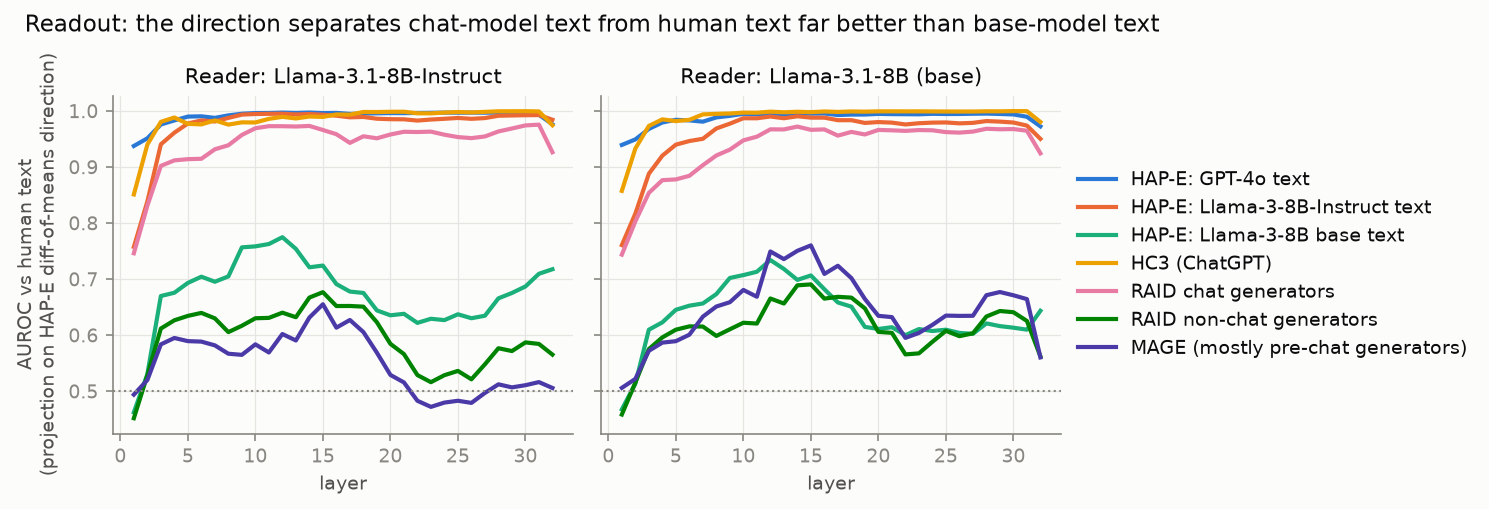
\includegraphics[width=0.95\linewidth]{figures/fig1_readout_by_layer.png}
\caption{AUROC of the projection on the \hape difference-of-means direction against human text, by layer and reading model. The direction separates chat-model text from human text almost perfectly from the early layers on and transfers to \hcthree and \raid chat generators. Text from base and pre-chat generators stays far lower at every layer.}
\label{fig:readout}
\end{figure}

\begin{table}[t]
\centering
\caption{Readout at layer 12: AUROC of the projection on \airead against human text. Rows in bold are generators that are not chat-tuned.}
\label{tab:readout}
\begin{tabular}{@{}lcc@{}}
\toprule
Test set & Instruct reader & Base reader \\
\midrule
\hape held-out, chat generators (diff-of-means / LR probe) & 0.996 / 1.000 & 0.991 / 0.999 \\
\hape GPT-4o text & 0.997 & 0.995 \\
\hape Llama-3-8B-Instruct text & 0.995 & 0.990 \\
{\bf \hape Llama-3-8B base text} & {\bf 0.775} & {\bf 0.734} \\
{\bf \hape Llama-3-70B base text} & {\bf 0.750} & {\bf 0.702} \\
\hcthree (ChatGPT vs.\ human answers) & 0.990 & 0.999 \\
\raid chat generators & 0.973 & 0.967 \\
{\bf \raid non-chat generators} & {\bf 0.640} & {\bf 0.665} \\
{\bf \mage (mostly pre-chat generators)} & {\bf 0.602} & {\bf 0.749} \\
Leave-one-genre-out, \hape (min--max over 6 genres) & 0.981--1.000 & 0.969--1.000 \\
\bottomrule
\end{tabular}
\end{table}

\Figref{fig:readout} and \tabref{tab:readout} reproduce the transferable direction of the probe literature.
\airead separates held-out chat-model text from human text at AUROC 0.996, holds up when a genre is left out (0.981--1.000), and transfers to \hcthree (0.990) and \raid chat generators (0.973).
Directions fitted on \hcthree and \raid reach 0.971 and 0.993 on \hape.

The same direction is weak for text that a model wrote without chat tuning: 0.75--0.78 for Llama-3 base text, 0.64 for \raid non-chat generators and 0.60 for \mage.
In human-SD units along the direction, chat-model texts sit at 4.4--4.8 and base-model texts at 1.0--1.1.
This is not an artifact of which generators were in the fit: a direction fitted on GPT-4o text only separates Llama-instruct text at 0.990 and Llama-base text at 0.674.
H1 therefore holds for chat-model text and fails as a statement about machine authorship.
The logistic-regression probe reads out slightly better and has cosine only 0.39 with \airead.

\subsection{Causal test: specific but partial}
\label{sec:causal}

\begin{figure}[t]
\centering
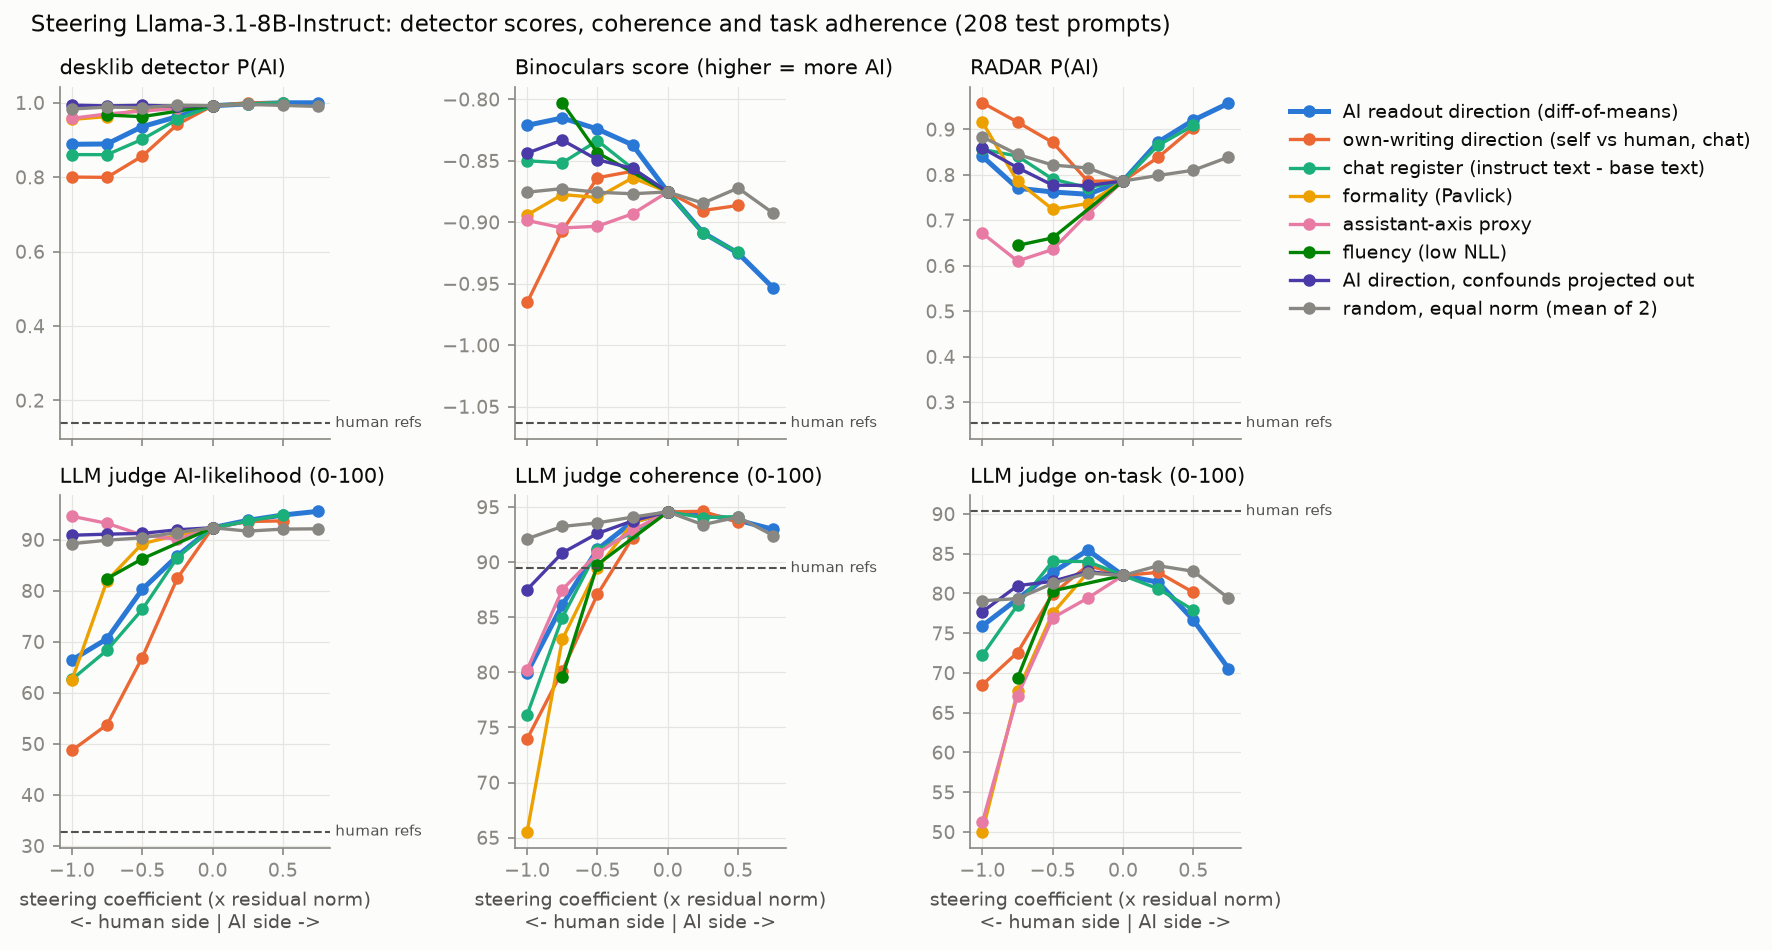
\includegraphics[width=\linewidth]{figures/fig3_dose_response.png}
\caption{Dose-response of steering \llamai at layer 12 on 208 test prompts. Negative coefficients steer toward the human side. The AI readout direction, the own-writing direction and the chat-register direction lower the judge's AI-likelihood and the \desklib score; the equal-norm random directions and the direction with confounds projected out do not. The \bino-style score moves the opposite way. Dashed lines mark human references.}
\label{fig:dose}
\end{figure}

\begin{table}[t]
\centering
\caption{Main steering results on 208 test prompts (layer 12). ``Flag'' is the share of texts above the 5\%-FPR threshold (\%). ``Sim'' is the embedding cosine with the unsteered output; ``RB'' is readback in human-SD units. Bold rows are the matched-coherence operating points of \airead and \writechat.}
\label{tab:main}
\resizebox{\textwidth}{!}{
\begin{tabular}{@{}lrcccccccccccc@{}}
\toprule
& & \multicolumn{2}{c}{Judge} & \multicolumn{2}{c}{\desklib} & \bino & \radar & \multicolumn{5}{c}{Quality and content} & \\
\cmidrule(lr){3-4}\cmidrule(lr){5-6}\cmidrule(lr){7-7}\cmidrule(lr){8-8}\cmidrule(lr){9-13}
Condition & $c$ & AI & flag & score & flag & flag & score & coher. & on-task & NLL & dist-3 & sim & RB \\
\midrule
Human references & & 32.8 & 3 & 0.139 & 5 & 5 & 0.25 & 89.4 & 90.3 & 2.68 & 0.99 & -- & 0.54 \\
Unsteered & & 92.4 & 99 & 0.992 & 100 & 83 & 0.79 & 94.6 & 82.3 & 1.48 & 0.98 & 1.00 & 4.35 \\
Unsteered, other seed & & 91.6 & 97 & 0.984 & 99 & 80 & 0.82 & 94.7 & 81.9 & 1.53 & 0.98 & 0.78 & 4.40 \\
Prompt ``write like a human'' & & 89.1 & 90 & 0.993 & 100 & 89 & 0.74 & 93.5 & 80.7 & 1.56 & 0.98 & 0.75 & 4.04 \\
Prompt ``write like an AI'' & & 94.2 & 100 & 0.997 & 100 & 75 & 0.84 & 94.4 & 80.6 & 1.47 & 0.98 & 0.80 & 5.05 \\
\midrule
\airead & $-0.25$ & 86.8 & 85 & 0.963 & 96 & 86 & 0.76 & 93.7 & 85.5 & 1.57 & 0.97 & 0.77 & 3.39 \\
\airead & $-0.50$ & 80.3 & 63 & 0.936 & 94 & 81 & 0.76 & 91.2 & 82.6 & 1.67 & 0.93 & 0.72 & 2.54 \\
{\bf \airead} & $\mathbf{-0.75}$ & {\bf 70.6} & {\bf 41} & {\bf 0.889} & {\bf 85} & {\bf 87} & {\bf 0.77} & {\bf 86.1} & {\bf 79.3} & {\bf 1.79} & {\bf 0.89} & {\bf 0.65} & {\bf 1.55} \\
\airead & $-1.00$ & 66.4 & 33 & 0.888 & 86 & 87 & 0.84 & 80.0 & 75.9 & 1.88 & 0.85 & 0.62 & 1.03 \\
\airead & $+0.25$ & 93.8 & 99 & 0.997 & 100 & 69 & 0.87 & 94.3 & 81.4 & 1.47 & 0.99 & 0.80 & 5.29 \\
\airead & $+0.50$ & 94.8 & 100 & 1.000 & 100 & 61 & 0.92 & 93.8 & 76.7 & 1.47 & 0.99 & 0.78 & 6.09 \\
\airead & $+0.75$ & 95.6 & 100 & 1.000 & 100 & 49 & 0.96 & 93.0 & 70.6 & 1.53 & 0.99 & 0.75 & 6.83 \\
\airead ablated, all layers & & 74.0 & 44 & 0.889 & 85 & 94 & 0.78 & 86.2 & 82.1 & 1.72 & 0.89 & 0.69 & 1.39 \\
\midrule
\writechat & $-0.25$ & 82.5 & 69 & 0.942 & 92 & 76 & 0.79 & 92.2 & 83.5 & 1.78 & 0.97 & 0.74 & 3.14 \\
{\bf \writechat} & $\mathbf{-0.50}$ & {\bf 66.9} & {\bf 35} & {\bf 0.857} & {\bf 82} & {\bf 76} & {\bf 0.87} & {\bf 87.1} & {\bf 79.9} & {\bf 2.16} & {\bf 0.94} & {\bf 0.65} & {\bf 1.70} \\
\writechat & $-0.75$ & 53.8 & 13 & 0.800 & 71 & 66 & 0.92 & 80.1 & 72.6 & 2.43 & 0.91 & 0.57 & 0.93 \\
\writechat ablated & & 65.7 & 26 & 0.764 & 69 & 86 & 0.75 & 83.6 & 81.4 & 2.14 & 0.93 & 0.68 & 1.34 \\
\ailr (probe weights) & $-0.75$ & 78.1 & 58 & 0.922 & 89 & 77 & 0.81 & 92.0 & 82.9 & 1.80 & 0.97 & 0.69 & 2.78 \\
\midrule
\dir{random0} & $-0.75$ & 91.5 & 95 & 0.995 & 100 & 81 & 0.85 & 93.3 & 81.2 & 1.49 & 0.97 & 0.78 & 4.37 \\
\dir{random0} & $-1.00$ & 90.7 & 94 & 0.987 & 99 & 78 & 0.90 & 92.5 & 80.0 & 1.54 & 0.97 & 0.77 & 4.33 \\
\dir{random1} & $-0.75$ & 88.3 & 87 & 0.982 & 99 & 75 & 0.84 & 93.2 & 77.5 & 1.69 & 0.98 & 0.72 & 4.02 \\
\dir{random0} ablated & & 91.1 & 95 & 0.994 & 100 & 79 & 0.81 & 93.7 & 82.3 & 1.49 & 0.98 & 0.81 & 4.44 \\
\bottomrule
\end{tabular}}
\end{table}

\Figref{fig:dose} and \tabref{tab:main} give the main run.

\para{What holds.}
{\em Dose-response in both signs.} Judge AI-likelihood, \desklib and readback fall monotonically with negative coefficients and rise with positive ones where there is headroom.
{\em Specificity.} Against the mean of the two random directions at the same coefficient, \airead at $c=-0.75$ changes the judge by $-19.3$ points (95\% CI $-22.8$ to $-15.7$) and \desklib by $-0.099$ ($-0.126$ to $-0.074$), both with Holm-corrected $p < 0.001$.
{\em Matched coherence.} \airead reaches $c=-0.75$ (coherence 86.1, on-task 79.3) with 41\% flagged by the judge and 85\% by \desklib. \writechat reaches $c=-0.5$ (coherence 87.1) with 35\% and 82\%. Random directions reach $c=-1.0$ with 85--94\% and 98--99\% (\figref{fig:frontier}).
{\em Better than prompting.} The ``write like a human'' prompt moves the judge by 3.3 points (CI 2.3--4.3) and does not move \desklib.
{\em Ablation.} Removing the direction at all layers gives judge 74.0 and \desklib flag 85\%; removing a random direction changes nothing.
{\em Closed loop.} Text written under steering re-reads at 1.55 SD, down from 4.35, so the intervention writes into the text the feature that the probe reads. Random steering leaves readback at 4.0--4.4.
{\em Not a length effect.} Steered outputs are shorter (140 to 117 words at $c=-0.75$). Truncating the unsteered outputs to the steered word counts leaves \desklib at 0.987 (steered: 0.889) and, on the 72 prompts judged before we reached an API limit, the judge at 93.0 (steered: 79.9 on the same prompts).
The effect is similar across tasks: $-22$, $-20$ and $-23$ judge points for \hape continuation, \hcthree answers and \raid writing.

\begin{figure}[t]
\centering
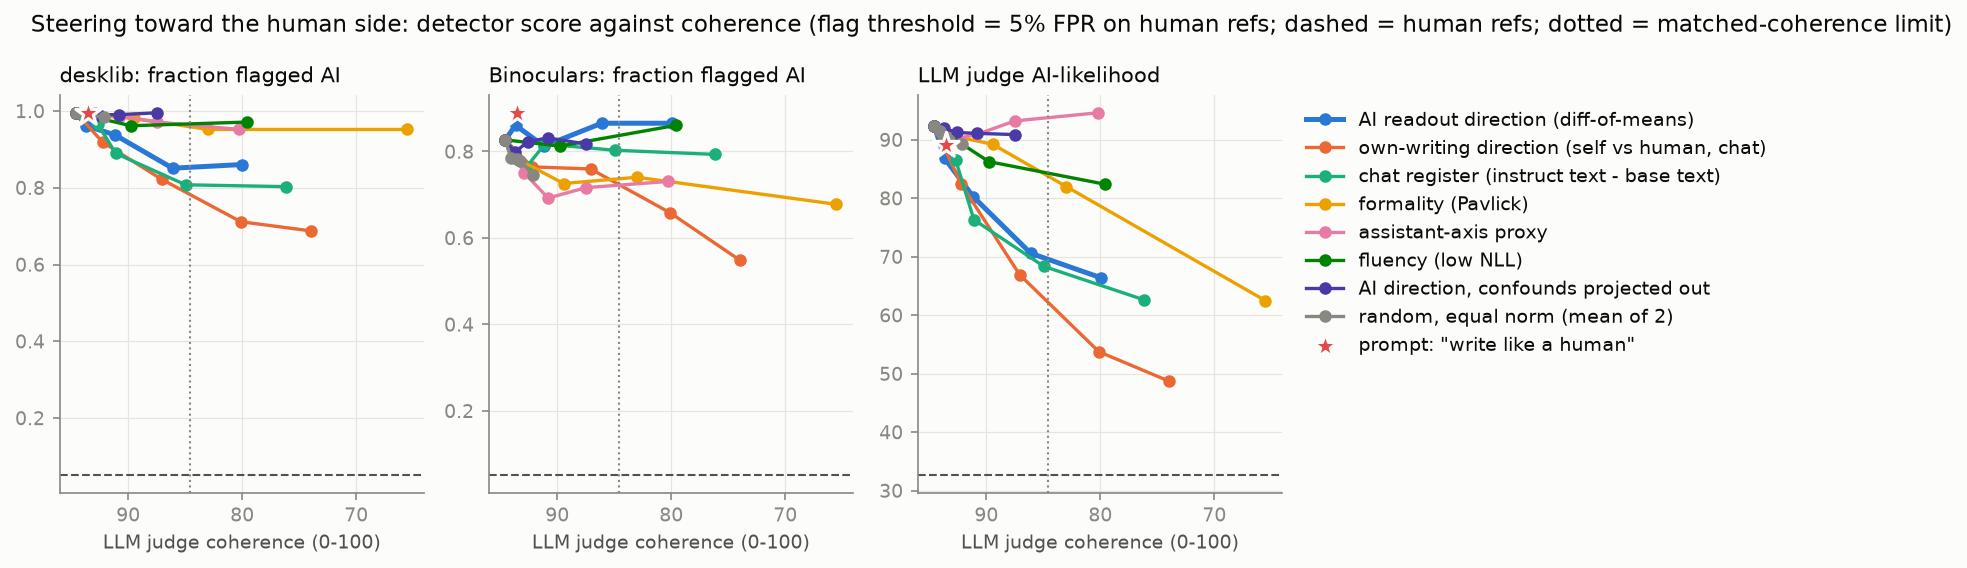
\includegraphics[width=\linewidth]{figures/fig4_frontier.png}
\caption{Detector score against judge coherence when steering toward the human side. Each line traces one direction over increasing $|c|$. The dotted line is the matched-coherence limit and the dashed line the human references. Only the AI readout, own-writing and chat-register directions lower the judge and \desklib before coherence is lost, and no direction comes near the human references on \desklib or \bino.}
\label{fig:frontier}
\end{figure}

\para{What does not hold.}
{\em Detector agreement.} \bino moves the wrong way: $+0.057$ against random at $c=-0.75$ (Holm $p<0.001$; 87\% flagged) and $-0.061$ at $c=+0.75$ (49\% flagged).
Over all 13{,}312 generated texts its Spearman correlation with the judge is $-0.24$ and with \desklib $-0.16$, although it separates unsteered output from human text at AUROC 0.93.
\radar does not differ from random on the human side (Holm $p = 0.60$).
The \hcthree RoBERTa score drops with steering (0.78 to 0.58), but the truncation control drops it as far (0.63), so we do not count it as evidence.
{\em Size.} At matched coherence the shift covers 37\% of the distance from unsteered output to human references on the judge and 12\% on \desklib. External NLL moves from 1.48 to 1.79, against 2.68 for human text.
{\em Content and quality.} Embedding similarity to the unsteered output falls from the seed-noise level of 0.78 to 0.65, distinct-3 falls from 0.98 to 0.89, and coherence drops 8.5 points. The output stays on task (79.3 vs.\ 82.3), but content is not held fixed.
{\em Positive side.} Steering toward AI lowers on-task scores (82.3 to 70.6 at $c=+0.75$) with coherence intact: on continuation prompts the model drifts into polished generic prose.

H2 is therefore partly supported: the direction is causal for how AI-like the text reads to a judge and, weakly, to the best supervised detector, but not for ``detected as AI'' in general.
\Tabref{tab:examples} shows typical outputs. Steered text is plainer and more colloquial, and its typical failure is looping.

\para{Readers vs.\ writers.}
The reading-derived direction controls writing, but less efficiently than the direction fitted on the model's own writing (\writechat: judge 66.9 at coherence 87.1, against 70.6 at 86.1).
The logistic-regression probe, the best reader, moves the judge least per unit norm among the three but preserves coherence best (78.1 at 92.0), in line with \citet{marks2023geometry}. We ran \ailr at two coefficients only, so its frontier is incomplete.

\begin{table}[t]
\centering
\caption{First lines of outputs for a \raid prompt asking for an IMDb review of {\em Vertigo}; the last row is a \hape fiction continuation that shows the typical failure (looping).}
\label{tab:examples}
\small
\begin{tabular}{@{}p{0.19\linewidth}p{0.77\linewidth}@{}}
\toprule
Condition & Output \\
\midrule
Unsteered & ``Alfred Hitchcock's `Vertigo' is a masterclass in suspense and psychological complexity. Released in 1958, this gripping thriller has stood the test of time\ldots'' \\
\airead, $c=-0.75$ & ``I just watched Vertigo for the third time and I still don't get it. I'm not saying that's a bad thing, I'm just saying that's what it's like. It's a masterful film by master filmmaker Alfred Hitchcock. He makes you think you know what's going on, then\ldots'' \\
\airead ablated & ``This is a very complex movie and I'm still not sure I completely understand it. The main character is a retired police officer who is a acrophobic (he is afraid of heights)\ldots'' \\
\airead, $c=+0.75$ & ``\ldots a masterclass in psychological suspense, weaving a complex web of obsession and deception that continues to captivate audiences to this day.'' \\
\airead, $c=-0.75$ (fiction) & ``It was a great comfort to him to be able to say with his eyes shut that the Lord had kept him from having a crop this year. It was a great comfort to him to be able to say that the Lord had kept him from having a crop next year\ldots'' \\
\bottomrule
\end{tabular}
\end{table}

\subsection{Disentanglement: the direction is chat register}
\label{sec:distinct}

\begin{figure}[t]
\centering
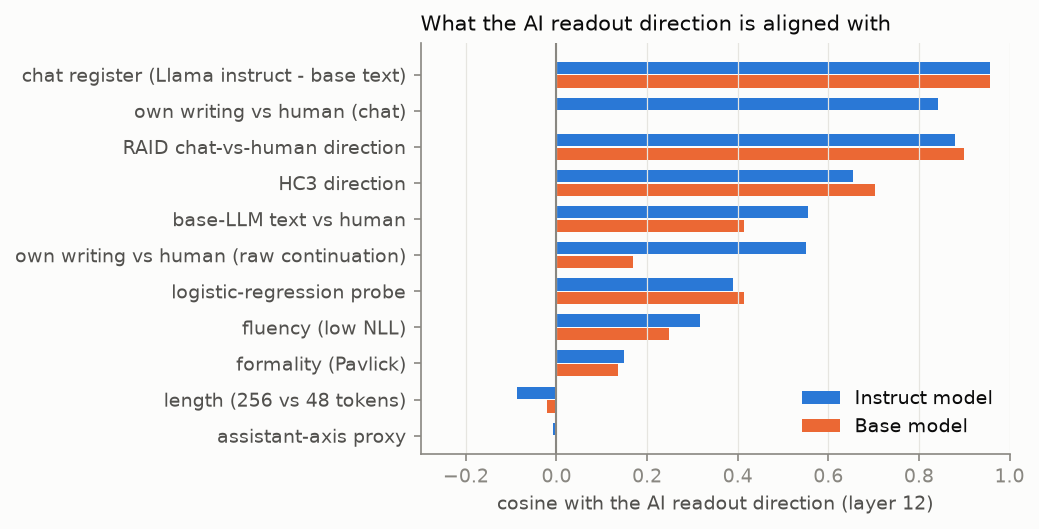
\includegraphics[width=0.8\linewidth]{figures/fig2_cosines.png}
\caption{Cosine of each candidate direction with the AI readout direction at layer 12, in both models. Chat register is almost parallel to it; formality, length and the assistant-axis proxy are close to orthogonal.}
\label{fig:cosines}
\end{figure}

\begin{table}[t]
\centering
\caption{Geometry at layer 12 of the instruct model. ``AUROC after removal'' is the held-out human-vs-chat AUROC after projecting the candidate out of the activations and refitting. ``Share removed'' is the share of \airead inside the candidate's span.}
\label{tab:geometry}
\resizebox{\textwidth}{!}{
\begin{tabular}{@{}lccc@{}}
\toprule
Candidate & Cosine with \airead & AUROC after removal & Share removed \\
\midrule
Chat register (Llama instruct $-$ base text) & {\bf 0.96} & {\bf 0.918} & {\bf 92\%} \\
Chat register, disjoint generators & 0.88 / 0.89 & -- & -- \\
Own writing vs.\ human, chat (\writechat) & 0.84 & -- & -- \\
Base-LLM text vs.\ human (\aibase) & 0.55 & -- & -- \\
Fluency (low NLL) & 0.32 & 0.996 & 10\% \\
Formality & 0.15 & 0.996 & 2\% \\
Length & $-0.09$ & 0.996 & 1\% \\
Assistant-axis proxy & $-0.01$ & 0.996 & $<0.1$\% \\
Genre subspace (5-D) & -- & 0.996 & 19\% \\
All of the above together & -- & 0.863 & 93\% \\
\bottomrule
\end{tabular}}
\end{table}

\para{Geometry.}
\Figref{fig:cosines} and \tabref{tab:geometry} show that \airead has cosine 0.96 with \chatreg, and that chat register accounts for 92\% of it.
The two directions share Llama-instruct texts, which inflates the cosine; with \airead fitted on GPT-4o text only and the register direction on the Llama 8B or 70B pair, it is 0.88--0.89.
Every other candidate is far from parallel: fluency 0.32, formality 0.15, length $-0.09$, assistant-axis proxy $-0.01$.
Projecting any of these out of the activations leaves the held-out AUROC at 0.996; projecting chat register out lowers it to 0.918.

Simple covariates do not explain the projection either.
The formality direction separates formal from informal sentences at AUROC 0.955 and human from AI text at 0.63, while \airead separates formal from informal sentences at 0.62.
NLL alone separates human from chat-model text at 0.89, but after regressing NLL and genre out of the projection, the projection still separates them at 0.957.
The Biber features \citep{biber1988variation} that correlate most with the projection are mean word length, nominalisations, prepositions, attributive adjectives and present participles (positive), and contractions, demonstrative pronouns, adverbs, second-person pronouns and emphatics (negative).
The same features order {\em human} texts along the direction ($r$ up to 0.60 and $-0.57$), so the direction is a property of the prose, with human text spread along it.

\begin{table}[t]
\centering
\caption{Steering with the candidate directions at equal norm (208 test prompts). Only directions that contain the chat-register component reproduce the effect of \airead on the judge and \desklib. ``Form.'' is the formality classifier score.}
\label{tab:candidates}
\resizebox{\textwidth}{!}{
\begin{tabular}{@{}lrccccccc@{}}
\toprule
Direction & $c$ & Judge AI & \desklib flag & \bino flag & Coher. & On-task & Form. & Readback \\
\midrule
Unsteered & & 92.4 & 100 & 83 & 94.6 & 82.3 & 0.81 & 4.35 \\
\airead & $-0.75$ & 70.6 & 85 & 87 & 86.1 & 79.3 & 0.81 & 1.55 \\
\chatreg & $-0.75$ & {\bf 68.4} & 81 & 80 & 85.0 & 78.5 & 0.86 & {\bf 1.28} \\
\midrule
\formality & $-0.50$ & 89.2 & 98 & 73 & 89.5 & 77.5 & 0.67 & 3.90 \\
\formality & $-0.75$ & 82.0 & 95 & 74 & 83.0 & 67.7 & 0.58 & 3.27 \\
\formality ablated & & 92.5 & 100 & 71 & 92.9 & 81.6 & 0.82 & 4.32 \\
\asstaxis & $-0.50$ & 90.9 & 99 & 69 & 90.8 & 76.9 & 0.72 & 4.40 \\
\asstaxis & $-0.75$ & 93.2 & 97 & 72 & 87.5 & 67.1 & 0.66 & 4.77 \\
\fluency & $-0.50$ & 86.3 & 96 & 81 & 89.8 & 80.3 & 0.65 & 3.43 \\
\lengthdir & $-0.50$ & 92.8 & 100 & 76 & 92.9 & 80.2 & 0.83 & 4.77 \\
\midrule
\perpall & $-1.00$ & 90.9 & 100 & 82 & 87.5 & 77.7 & 0.74 & 3.65 \\
\perppersona & $-0.75$ & 90.7 & 98 & 80 & 89.9 & 79.7 & 0.70 & 3.87 \\
\midrule
\aibase & $-0.75$ & 79.8 & {\bf 74} & {\bf 58} & 87.8 & 84.4 & 0.76 & 2.63 \\
\aihc & $-0.50$ & 72.1 & {\bf 74} & 73 & 88.4 & 82.6 & 0.76 & 2.32 \\
\bottomrule
\end{tabular}}
\end{table}

\para{Steering with the candidates.}
\Tabref{tab:candidates} gives the causal counterpart.
{\bf Formality is not it.} Steering toward informal lowers the formality classifier score (0.81 to 0.58), but the judge moves only when coherence collapses (at $c=-1.0$: judge 62.5 with coherence 65.5 and on-task 50.0). \airead leaves the formality score unchanged.
{\bf The assistant-axis proxy is not it.} Moving away from the assistant pole leaves the judge at 91--95 and \desklib unchanged while on-task falls to 51 at $c=-1.0$. It does lower \radar (0.79 to 0.61).
{\bf Chat register is it.} \chatreg steers like \airead (judge 68.4, \desklib flag 81\%). With the chat-register span removed (\perppersona, \perpall), the direction does nothing to the judge or \desklib, even at $c=-1.0$.

H3 is therefore refuted for chat register and supported for formality, fluency, length, genre and the assistant-axis proxy.

\para{A second axis.}
\aibase (base-LLM text minus human text; cosine 0.55 with \airead) is the only direction that lowers the \bino flag rate (83\% to 58\%), and it raises external NLL the most (2.35).
It also lowers \desklib more than \airead at similar coherence.
This is one run of one direction, and we did not test what it encodes.
\aihc, fitted on the confounded \hcthree contrast, also moves the judge and \desklib more than \airead at similar coherence, but it mixes register with whatever else separates Reddit answers from ChatGPT answers, so we cannot attribute its effect.

\subsection{Base vs.\ instruct: the direction pre-exists chat tuning}
\label{sec:base}

\begin{table}[t]
\centering
\caption{Base and instruct models compared at layer 12. Offsets are along each model's own direction in human-SD units.}
\label{tab:baseinstruct}
\begin{tabular}{@{}lcc@{}}
\toprule
Quantity & Base model & Instruct model \\
\midrule
Held-out AUROC, chat-model vs.\ human text & 0.991 & 0.996 \\
Offset of chat-model text & 5.6--6.9 & 4.4--4.8 \\
Offset of base-LLM text & 0.8--1.0 & 1.0--1.1 \\
Cosine between the two models' directions & \multicolumn{2}{c}{0.84 (0.87 at layer 16)} \\
Base direction applied to instruct activations, AUROC & \multicolumn{2}{c}{0.996} \\
Own writing vs.\ human, raw prefix (offset / AUROC) & 0.45 / 0.62 & 1.39 / 0.78 \\
Own writing vs.\ human, chat template (offset / AUROC) & -- & 3.89 / 0.99 \\
Readback of own test output, raw continuation & 0.82 & 1.79 \\
Readback of own test output, chat & -- & 4.35 \\
\bottomrule
\end{tabular}
\end{table}

\Tabref{tab:baseinstruct} shows that the base model has the same direction with the same readout quality (AUROC 0.991; cosine 0.84 with the instruct model's direction), so the direction is learned from pretraining text and is not created by chat tuning.
The separation is, if anything, larger in the base model.
What chat tuning changes is where the model writes: almost at the human position for the base model (0.45 SD), partly shifted for the instruct model continuing raw text (1.39 SD), and at the chat-model position under the chat template (3.89 SD).
The mean activation shift from base to instruct on identical text is not along the direction (cosine $-0.19$).

\begin{figure}[t]
\centering
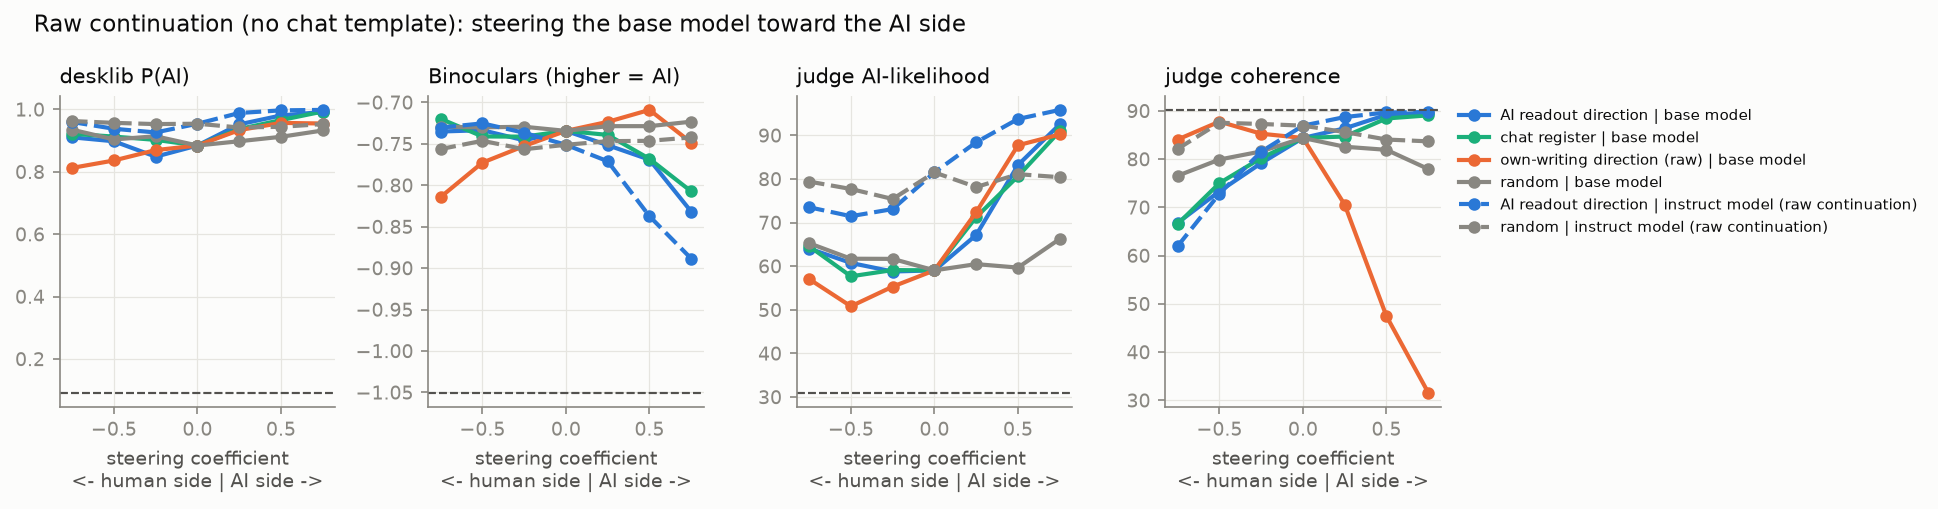
\includegraphics[width=\linewidth]{figures/fig5_base_model.png}
\caption{Steering raw continuation (150 \hape prefixes, no chat template). Adding the AI readout or chat-register direction to the base model raises the judge's AI-likelihood to the level of chat-model output while judged coherence rises. Random directions do not. Dashed horizontal lines mark human continuations.}
\label{fig:base}
\end{figure}

\begin{table}[t]
\centering
\caption{Steering raw continuation in the base and instruct models (150 \hape prefixes). \desklib and \bino are near ceiling here, so the result rests on the judge.}
\label{tab:basecont}
\resizebox{\textwidth}{!}{
\begin{tabular}{@{}llrccccccc@{}}
\toprule
Model & Condition & $c$ & Judge AI & \desklib & \bino flag & Coher. & On-task & Dist-3 & Readback \\
\midrule
-- & Human continuation & & 31.0 & 0.092 & 5 & 90.2 & 96.3 & 0.99 & 0.12 \\
\midrule
Base & Unsteered & & 59.0 & 0.884 & 97 & 84.4 & 87.0 & 0.86 & 0.82 \\
Base & \airead & $+0.25$ & 67.2 & 0.952 & 95 & 86.4 & 86.2 & 0.92 & 1.56 \\
Base & \airead & $+0.50$ & 83.2 & 0.981 & 95 & 89.2 & 81.6 & 0.95 & 2.99 \\
Base & \airead & $+0.75$ & {\bf 92.5} & 0.992 & 89 & {\bf 89.6} & 71.7 & 0.98 & 5.71 \\
Base & \chatreg & $+0.75$ & 91.0 & 0.993 & 97 & 89.1 & 73.7 & 0.97 & 4.80 \\
Base & \dir{random0} / \dir{random1} & $+0.75$ & 67.4 / 65.1 & 0.942 / 0.923 & 98 / 99 & 76.5 / 79.4 & 81.0 / 83.7 & 0.79 / 0.85 & 0.93 / 0.80 \\
Base & \airead & $-0.50$ & 60.7 & 0.898 & 95 & 73.3 & 78.0 & 0.76 & 0.17 \\
Base & \writeraw & $-0.50$ & 50.8 & 0.836 & 97 & 87.8 & 91.3 & 0.94 & 0.64 \\
Base & \writeraw & $+0.50$ & 87.7 & 0.957 & 91 & 47.4 & 55.4 & 0.45 & 0.36 \\
\midrule
Instruct & Unsteered & & 81.5 & 0.954 & 97 & 86.9 & 84.7 & 0.91 & 1.79 \\
Instruct & \airead & $+0.50$ & 93.8 & 0.997 & 93 & 89.7 & 74.5 & 0.98 & 4.36 \\
Instruct & \airead & $-0.50$ & 71.5 & 0.938 & 98 & 72.8 & 78.2 & 0.75 & 0.43 \\
\bottomrule
\end{tabular}}
\end{table}

\para{Steering the base model.}
\Figref{fig:base} and \tabref{tab:basecont} show that adding the direction to the base model raises the judge's AI-likelihood from 59.0 to 92.5 at $c=+0.75$: 26.3 points over random (Holm $p<0.001$), and 23.5 at $c=+0.5$.
Judged coherence {\em rises} ($+7$ to $+12$ over random) and repetition falls.
The base model starts writing in chat-model register.
Subtracting the direction does nothing to the judge, since the base model is already near the human position, and costs coherence.
The base model's own-writing direction (\writeraw, cosine 0.17 with \airead) is a different thing: adding it produces repetition collapse (distinct-3 0.45, external NLL 1.13), and subtracting it raises NLL and coherence and lowers the judge by 11 points over random.
H4 is supported.

\para{An unexpected baseline.}
Unsteered base-model continuations are flagged by \desklib (92\%) and \bino (97\%), unlike the 97--99\% ``human'' rates that \citet{xu2026base} report for GPTZero and Pangram.
Our continuations were sampled at temperature 0.7 and are repetitive (distinct-3 0.86; external NLL 1.80 vs.\ 2.87 for human text), whereas \citet{xu2026base} sample at temperature 1.0.
We did not rerun at 1.0, so the cause is not established.

\section{Discussion}
\label{sec:discussion}

\para{What ``sounding like AI'' is in this model.}
The direction that the probe literature reads as machine authorship is, in \llamai, the difference between how chat-tuned models write and how base models and humans write: longer words, nominalisations, participial and prepositional phrases, and few contractions.
It is not ``written by a model'', because base-model text barely moves along it.
It is not ``being the Assistant'', because the persona proxy is orthogonal to it and steering along the proxy leaves AI-likeness unchanged.
And it is not created by chat tuning: the base model already has it, and chat tuning together with the chat template sets where the model's own writing sits on it.

\para{Implications for detection.}
Activation-probe detectors of the kind in the literature are, in this model, detectors of chat-model register.
This explains both their strong transfer across chat generators and their weakness on non-chat generators, which \citet{vishnyakov2026svdetect} observed on \raid, and it gives a geometric reading of the behavioural result of \citet{xu2026base}.
It also means the same vector is a style control and not an authorship variable.
As an evasion tool it is poor: at preserved coherence the best supervised detector still flags 85\% of texts and the perplexity-based detector flags more, not fewer.

\para{The \bino reversal.}
We have no tested explanation.
Three observations bear on it: steering toward the human side raises external NLL only slightly while lowering lexical diversity; steering toward the AI side lowers the \bino flag rate with NLL unchanged; and the one direction that lowers \bino (\aibase) is the one that raises NLL most.
These are consistent with \bino tracking predictability and not register, which would make register and predictability two separate axes of ``AI-likeness''.
The experiments that would show this, such as steering both directions jointly or scoring with the original Falcon pair, were not run.

\para{Surprises.}
Removing the chat-register component leaves a vector that still reads back as slightly less AI (3.65 SD) but has no detector or judge effect.
Base-model continuations at temperature 0.7 are heavily flagged by perplexity-based and supervised detectors.
And steering toward AI raises judged coherence in the base model.

\para{Limitations.}
{\em Scope.} We study one model family, steer at one layer chosen on dev prompts, and use one sampling seed per condition (seed-to-seed differences of the unsteered condition are at most 0.7 judge points and 0.01 on \desklib).
{\em The judge may share the confound.} An LLM judge asked for AI-likelihood may itself key on chat register. Its agreement with \desklib (Spearman 0.56 over all generated texts) and its AUROC of 0.99 on human vs.\ model text argue that it measures something real, but the headline effect is largest on the measure most likely to be register-sensitive. About 3\% of judge calls hit the primary model's content filter and were scored by a second model, and one main-run item has no judge score.
{\em \bino is non-standard.} We use a Qwen2.5-7B pair, not the Falcon pair of \citet{hans2024binoculars}. It validates at AUROC 0.93 on our prompts, but the reversal should be checked with the original models and with a commercial detector; none was accessible.
{\em Incomplete truncation control.} The judge half of the length control covers 72 of 208 prompts (all 208 for \desklib).
{\em Assistant-axis proxy.} We use 40 roles with 8 questions each and no judge filtering, not the 275-role pipeline of \citet{lu2026assistant}; a null for the proxy is weaker than a null for the real axis.
{\em Shared generators.} The 0.96 cosine with chat register is inflated by shared Llama-instruct texts; the disjoint-data value is 0.88--0.89.
{\em References.} Human references are not length-matched to generations (175 vs.\ 140 words on average), and \hcthree human answers carry tokenisation artifacts, so the detector validation AUROCs are optimistic.
{\em Intervention design.} We tested only mean-pooled directions added at all positions, and ran the second-tier directions (\ailr, \fluency, \lengthdir, \perppersona, \aibase, \aihc) at two coefficients only.
{\em Statistics.} Holm correction applies within each metric across the conditions of a run; the descriptive comparisons elsewhere are uncorrected.
\Secref{app:details} lists deviations from the pre-specified plan.

\section{Conclusion}
\label{sec:conclusion}

\llamai has a linear direction that makes its output read as more or less AI-written, and the direction is causal in both the instruct and the base model.
It is not an authorship variable and not the assistant persona.
It is the prose register of chat-tuned models, already present in the base model, onto which chat tuning moves the model's default writing.
Moving along it changes an LLM judge's impression substantially (92.4 to 70.6 at matched coherence) and a supervised detector slightly (99.5\% to 85\% flagged), and does not make the text statistically human-like to a perplexity-based detector.

Several follow-ups would sharpen this picture.
The first is to test the two-axis reading directly by steering \airead and \aibase jointly and checking whether judge, supervised and perplexity-based detectors all move at preserved coherence.
The second is to rerun the base-model baseline at temperature 1.0 and score it with the original \bino pair and a commercial detector, to resolve the disagreement with \citet{xu2026base}.
Beyond these, the result needs replication on a second model family and with the real Assistant Axis, human raters to check the judge, and a sparse-autoencoder decomposition to see whether the direction is one feature or the sum of the verbosity, hedging and complexity features that \citet{kuznetsov2025sae} list.


\bibliography{references}

\appendix
\section{Additional Details}
\label{app:details}

\begin{table}[h]
\centering
\caption{Definitions of all directions. Each is a unit vector at layer 12.}
\label{tab:directions}
\small
\begin{tabular}{@{}lp{0.72\linewidth}@{}}
\toprule
Name & Definition \\
\midrule
\airead (primary) & mean(chat-generator texts) $-$ mean(human continuations), \hape fitting split \\
\ailr & logistic-regression probe weights on the same data \\
\writechat & the instruct model's own response activations $-$ the matched human reference teacher-forced in the same assistant slot (455 fit prompts) \\
\writeraw & own raw continuation $-$ true human continuation after the same prefix \\
\chatreg & Llama-3-8B/70B-Instruct texts $-$ Llama-3-8B/70B base texts (\hape) \\
\aibase & base-LLM texts $-$ human texts \\
\aihc, \dir{ai\_raid} & the \airead contrast fitted on \hcthree / \raid chat generators \\
\formality & formal $-$ informal sentences of \citet{pavlick2016formality}, top vs.\ bottom quintile (900 + 900) \\
\fluency & low-NLL $-$ high-NLL terciles of human texts (NLL under the reading model) \\
\lengthdir & 256-token pooling $-$ 48-token pooling of the same human texts \\
\asstaxis & default-assistant responses $-$ mean of 40 role-play personas (roles and questions from the Assistant Axis repository; 8 questions per role; no judge filtering) \\
\dir{random0/1} & fixed Gaussian directions \\
\perpall & \airead with the span of formality, fluency, length, chat register, assistant axis and the 5-D genre subspace projected out \\
\perppersona & \airead with chat register and assistant axis projected out \\
\bottomrule
\end{tabular}
\end{table}

\para{Prompt baselines.}
The ``human'' system prompt reads: ``Write like a human, not like an AI. Your text must read as if a real person wrote it: natural and unpolished where appropriate, with none of the phrasing, structure or tone typical of AI assistants.''
The counterpart asks for ``unmistakable AI assistant style''.

\para{Layer and coefficient selection.}
We compared layers 8, 12, 16 and 20 on the 89 dev prompts using \desklib, external NLL and distinct-3, and chose layer 12 and the coefficient grid $\{0.25, 0.5, 0.75, 1.0\}$ there.

\para{Implementation.}
Python 3.12.8, torch 2.6.0 and transformers. The seed for data splits is 42, and generation seeds are fixed per batch.
Generation uses batches of 50--104 and activation extraction batches of 32--48.
Activation extraction takes about 20 minutes per model, the main steering run about 2 hours 10 minutes, and scoring about 50 minutes.

\para{Judge.}
The judge is \texttt{openai/gpt-5.6-terra} via OpenRouter at temperature 0, blind to condition.
About 3\% of calls hit its content filter and were scored by \texttt{anthropic/claude-sonnet-5} instead.
The run made about 20{,}100 unique judge calls (about 11.2M input and 1.2M output tokens).
The API key reached its daily spending limit near the end of the run; the only analysis affected is the judge half of the truncation control.

\para{Deviations from the plan.}
We dropped a third random direction and a formality-only residualised direction for time.
We tightened the matched-coherence rule to require the on-task score to be within 10 points as well.
A logit-lens reading of the layer-12 directions returned uninterpretable tokens and is not used.


\end{document}
